    \documentclass[12pt,twoside]{report} % Use esta linha para tese com mais de 100 p{\'a}ginas
%    \documentclass[12pt]{report} % Use esta linha para tese com at{\'e} 100 p{\'a}ginas

    \usepackage{ic-tese}
    \usepackage[latin1]{inputenc}
    \usepackage[brazil]{babel}
    \usepackage{my-ic-tese}

    \usepackage{latexsym}
    \usepackage{amssymb,amsmath,latexsym,amsfonts}
    \usepackage{graphicx}
    \usepackage{subfig}
    \usepackage{makeidx}



    \begin{document}
    \title{Estudo e Implementa��o de Mecanismos de Codifica��o por Apagamento no Hadoop \emph{File System}}
    \author{Celina d'�vila Samogin}
    \degreesought{Mestrado} % Doutorado
    \titlesought{Mestre}     % Doutora/Mestre
    \principaladvisor{Profa. Dra. Islene Calciolari Garcia}
    \advisortitle{Orientadora} % Orientadora
%    \coadvisor{Byron Meter (Co-orientador)} % Pode ser omitido.
    \firstreader{Prof. Ph.D. Luiz Eduardo Buzato}
    \secondreader{Prof. Ph.D. Ricardo Dahab}
    \thirdreader{Prof. Dr. Edmundo Roberto Mauro Madeira (suplente)}
%    \fourthreader{Fairy Tail}
    \grants{{\rm Suporte financeiro de: Bolsa do CNPq (processo XYZ) 2010--2010.}} % Pode ser omitido.
%
    \submitdate{30 de Janeiro de 2012} % Pode ser omitido.
    \date{05 de Mar�o de 2012} % Pode ser omitido.
%
%   Se pretende utilizar \copyrighttrue, consulte antes seu orientador ou a CPG!!!
%   Este ponto envolve quest{\~o}es legais complexas e de graves conseq{\"u}{\^e}ncias.
    \copyrightfalse % Caso nao queira que apareca a pagina de Copyright.
%    \copyrighttrue % Caso queira que apareca a pagina de Copyright.
%
%    \finalversiontrue % Caso seja a versao final.
    \finalversionfalse % Caso nao seja a versao final ainda.
%
    \tablespagetrue % Caso queira que apareca a Lista de Tabelas.
%    \tablespagefalse % Caso nao queira que apareca a Lista de Tabelas.
%
    \figurespagetrue % Caso queira que apareca o Lista de Figuras.
%    \figurespagefalse % Caso nao queira que apareca o Lista de Figuras.
%
    \beforepreface
    \prefacesection{Resumo}
    \begin{abstract}
  Os dados em um sistema distribu�do confi�vel devem estar dispon�veis
  quando for necess�rio. A codifica��o por apagamento (\emph{erasure
    codes}) tem sido utilizada por sistemas para alcan�ar requisitos
  de confiabilidade e de redu��o do custo de armazenamento de dados. O
  Hadoop � um \emph{framework} para execu��o de aplica��es em
  armazenamento distribu�do de grande volume de dados e que pode ser
  constru�do com \emph{commodity hardware}, que � facilmente acess�vel
  e dispon�vel. Esta proposta apresentar� uma an�lise da viabilidade
  da implementa��o pr�tica de t�cnicas de codifica��o por apagamento
  no Hadoop \emph{Distributed File System} (HDFS), as altera��es no
  Hadoop e a efic�cia dessas altera��es. Esta proposta � uma
  contribui��o para \emph{software} livre em sistemas distribu�dos.
\end{abstract}

\begin{center}
{\bf Abstract}
\end{center}

%% \begin{abstract}
 The data in a reliable distributed system should be available when needed. Erasure codes have been used by systems to meet reliability requirements and reduce the cost of data storage. The Hadoop is a framework for running applications on distributed storage of large volumes of data and it can be built with commodity hardware, which is easily accessible and available. This proposal will examine the feasibility of practical implementation of erasure coding techniques in Hadoop File System (HFS), changes in Hadoop and effectiveness of those changes. This proposal is a contribution to free software in distributed systems.
%% \end{abstract}

 
    \prefacesection{Abstract}
    %\chapter*{Abstract}\label{ch:abstract}
  The data in a reliable distributed system should be available when
  needed. Erasure codes have been used by systems to meet reliability
  requirements and reduce the cost of data storage. The Hadoop is a
  framework for running applications on distributed storage of large
  volumes of data and it can be built with commodity hardware, which
  is easily accessible and available. This dissertation presents theorical
  aspects involved and a practical implementation of erasure coding techniques
  in Hadoop Distributed File System (HDFS), changes in Hadoop and
  effectiveness of those changes. This work is a contribution to
  free software in distributed systems.

    \prefacesection{Agradecimentos}
    %\chapter*{Acknowledgements}
Agradeço minhas irmãs Eunice e Helena, que sempre me apoiaram nas minhas conquistas (foram muitas) e nos meus fracassos (foram poucos) e meus filhos Paula, Carolina e Daniel que entenderam minha ausência. Meus tios e tias, meus primos e primas também sempre me apoiando, querendo saber das novidades e perguntando: "quando você vem em Lins ?". A família é mesmo minha fortaleza.

Meus queridos amigos de quatro patas também tiveram muito a ver com esse trabalho. Uma parte da viabilização do trabalho foi obtida do faturamento das aulas de adestramento para cães e gatos que eu fiz entre 2005 e 2009. Depois disso, eu me afastei do trabalho com proprietários e continuei com o trabalho voluntário para as ONGs de posse responsável e castração, continuando a treinar animais resgatados das ruas para que eles ficassem mais adotáveis. A profa Maria de Fátima Martins (USP-FMVZ) e suas alunas Msc. Michele Ribeiro Silva e Msc. Juliana de Vazzi Pinheiro também foram muito importantes nesse processo difícil de voltar a academia. Ela me aconselhava em conversas: "Ela não tem que fazer outra faculdade!".

O colega de turma e amigo Paulo Cezar Campioni também apoiou meu trabalho de mestrado. Foi um pai sempre presente com nossos filhos.

Agradeço ao CNPq (Conselho Nacional de Desenvolvimento Científico e Tecnológico) pelo apoio concedido no início do meu mestrado e a FAPESP (Fundação de Amparo à Pesquisa do Estado de São Paulo) pelo apoio concedido ao meu projeto "Desenvolvimento e Qualidade de Dados para Sistema de Informação de Biodiversidade (Projeto de Pesquisa: Desenvolvimento de novas ferramentas e migração dos sistemas BIOTA do CRIA para o CENAPAD/UNICAMP)".

Agradeço aos professores, membros da banca. É uma honra contar com suas contribuições para meu trabalho.

O meu agradecimento também vai para os coordenadores de graduação e pós-graduação do IC, nesse período de 2010 a 2011, profo Ricardo da Silva Torres, profo Sandro Rigo, profo Hélio Pedrini, profo Alexandre Xavier Falcão e profo Paulo Lício de Geus.

Eu não queria falar muito do passado, mas eu tentei iniciar no programa de pós-graduação, logo que eu terminei a graduação em 1985 e uma outra vez, em 2002. Eu acredito que viram meu potencial, pois me aceitaram pela terceira vez no IC em 2010 e eu pude, então, concluir o programa de mestrado.

Também gostaria de agradecer minha colega e amiga Claudia Marconi Engler Pinto, da turma de ciência da computação de 1981, pela palestra sobre Unix, ocorrida um tempo depois da minha formatura na graduação, que me despertou o interesse por esse sistema operacional. Ao CPqD Telebrás, hoje, Fundação CPqD, por ter me oferecido a oportunidade de assistir a palestra apresentada pela colega Claudia e de cursar disciplinas do Laboratório A-HAND, na época com o coordenador, o profo Rogério Drummond, onde eu pude aprender, com muita qualidade, a programar em sistemas Unix, muito antes de eu conhecer o sistema Linux e os sistemas MS Windows.

Já algum tempo, antes de 2008, quando eu quis aprender a teoria de computação que estava sendo oferecida nos cursos de graduação do IC, as páginas dos cursos do profo Rezende foram (e continuam a ser) importantes fontes de informação sobre essa área e me ajudaram muito a direcionar meus estudos. Obrigada, professor Rezende, por me aceitar como ouvinte nas disciplinas de Fundamentos Matemáticos da Computação (MC348) e Projeto e Análise de Algoritmos I (MC448), por proporcionar aulas tão bem elaboradas, lousas perfeitas e por demonstrar sempre disposição com as dúvidas que você me respondeu nos horários de atendimento. Fazer os quase 500 exercícios propostos nessas aulas me prepararam para as disciplinas da pós-graduação.

Também não posso me esquecer dos colegas de ciência da computação de 2007 que me adotaram como parte da turma, afinal, além das disciplinas com o profo Rezende, eu assisti Banco de Dados (MC536) com eles também! As animadas e surpreendentes aulas da profa Claudia também me prepararam para a pós. Obrigada Alex Grilo, Michael, Vanessa Schissato, Douglas Drummond, Bruno Malveira, Guilherme Paulovic, Guilherme Sampaio, Helen Her, Bráulio, "Panda" e demais colegas, que eu lembro a fisionomia, mas não anotei o nome.

Agradeço também o profo Meidanis por me fazer estudar todos os dias nos meses de aulas de Complexidade de Algoritmos I (MO417). As técnicas utilizadas e o formato das aulas e das avaliações exigiram de mim mais participação na disciplina e diminuíram meu estresse com relação aos tópicos da disciplina. Foi uma boa convivência com meus colegas dessa turma também. Não teve turma mais legal!

Entre outras coisas, a profa Ariadne e o profo Buzato me ensinaram como registrar e escrever resumos de artigos, que "comunicam em uma página a tese apresentada pelos autores e a sua relevância", o que é essencial para o desenvolvimento do trabalho da pós-graduação. Agradeço muito a eles por isso.

A oferta da disciplina Projeto e Implementação de Sistemas Distribuídos (MO641) pelo profo Buzato com trabalhos e seminários focados no projeto do Hadoop, também foi muito importante, pois pude conhecer e implementar aplicações que esse sistema distribuído de arquivos pode suportar.

Com o apoio da docente, a Profa Islene, minha orientadora, eu tive uma boa e interessante experiência para minha carreira de docente no estágio PED da disciplina Laboratório de Sistemas Distribuídos (MC715). Aprendi muito assistindo as apresentações dos alunos, inclusive como capturar imagem do monitor para criar um vídeo e instalando, compilando e testando o código java dos projetos dos alunos no Cluster do IC!

Obrigada Profa Islene, que sempre acreditou no meu potencial e me conduziu durante o mestrado. Pela sua atenção, paciência, experiência, tranquilidade, sorrisos, incentivo e críticas que contribuíram para o meu crescimento como aluna e como pessoa. Foi um grande privilégio tê-la como orientadora.

Não poderia deixar de agradecer o profo Tomasz pelas ótimas aulas que assisti na disciplina Estrutura de Dados (MC202) no programa de estágio PED e por ele sempre mostrar tanta qualidade e entusiasmo como professor. Responder as dúvidas no laboratório e por e-mail e fazer uma avaliação das tarefas dos alunos da turma de ciência da computação de 2011, com ajuda do colega Thiago Cavalcante, me estimularam a desenvolver técnicas para meu aprimoramento como docente.

Agradeço muito ao Rodrigo Schmidt do Facebook, ex-aluno do IC, pelas sugestões de temas, das quais escolhi \emph{erasure coding} e pela sua disposição em responder minhas dúvidas sobre a camada RAID do Hadoop. Não foi só ele que me ajudou nessa tarefa de conhecer o Hadoop. Também agradeço Scott Chen e Ramkumar Vadali.

Com a muito competente equipe da secretaria de pós-graduação, Daniel Capeleto, Fernando Okabe, Wilson Bagni Junior e Ademilson Ramos dos Reis, meu período como aluna no IC foi muito tranquilo. Pude contar com eles para todo apoio e para resolver qualquer problema.

Também quando um apoio de informática foi importante, Wiliam Lima Reiznautt e sua equipe sempre estavam dispostos a resolver a questão.

Sem música, alguns dias teriam sido muito difícies. Obrigada Paralamas do Sucesso, Skank, Legião Urbana, Capital Inicial, Tim Maia, Erasmo Carlos, Mutantes, Rita Lee, Celly Campello, Raul Seixas, Elis Regina, Nara Leão, João Gilberto, Chico Buarque, Paulinho da Viola, Demônios da Garoa, Carlos Lyra, Tom Jobim, Vinicius de Moraes, Tiê, Trio Irakitan, Almir Sater, Cascatinha e Inhana, Fafá de Belém, Marisa Monte, Arnaldo Antunes,  Adriana Calcanhoto, Renato Russo, Pepeu Gomes, Caetano Veloso, Gilberto Gil, Léo Jaime, Cazuza, Metrô, Premeditando o Breque, Lobão, Camisa de Vênus, Ira!, Roupa Nova, 14 Bis, Blitz, Kid Abelha, Morris Albert, Norah Jones, Aretha Franklin, B. J. Thomas, Nat King Cole, Elvis Presley, Chuck Berry, Jerry Lee Lewis, Roy Orbison, Frank Sinatra, The Platters, Bob Dylan, Al Stewart, Cat Stevens, The Beatles, Suzi Quatro, Rolling Stones, Supertramp, Aerosmith, Nirvana, Led Zeppelin, Talking Heads, Sixpence None the Richer, Five, Dire Straits, Aqualung, The Police, The Who, REM, Duran Duran, Peter Frampton, Art Garfunkel, John Lennon, Paul McCartney, George Harrison, Ringo Star, Paul Simon, David Bowie, Carlos Santana, Eric Clapton, Elton John, Carly Simon, Jack Johnson, Lynyrd Skynyrd, Beach Boys, Player, Three Dog Night, The Eagles, The Doors, Amy Winehouse, Bread, Carpenters, The Mamas and The Papas, Joan Baez, Lobo, The Monkees, Pink Floyd, The Alan Parsons Project, Nicolette Larson, Kate Bush, Laura Pausini, Dolly Parton, Earth, Wind and Fire, Michael Jackson e Avril Lavigne pela voz, letras e melodias e muitos outros artistas pelas músicas com arranjos para violão, gaita de fole e saxofone e com solos de guitarra.

Agradeço ainda toda comunidade de software livre por todas as informações que pude encontrar nos fóruns, nas listas de discussão, nos sites, nas documentações, por toda a conquista do software de qualidade obtida com o trabalho colaborativo, software esse testado por milhares de pessoas e em centenas de projetos e empresas. É nisso que eu acredito!




    \prefacesection{ }
    %\chapter*{}
\begin{center}
{\centering \it Dedico ao meu pai Ant�nio (in memoriam), � minha m�e Maria (in memoriam), �s pessoas que, de alguma maneira, com suas atitudes, contribu�ram para a realiza��o deste trabalho e a todos que dedicam sua vida a pesquisa cient�fica.}
\end{center} 

    \prefacesection{ }
    %\chapter*{}
\vspace{14cm}
{\it Há homens que lutam um dia, e são bons; há outros que lutam um ano, e são melhores; há aqueles que lutam muitos anos, e são muito bons.
Porém há os que lutam toda a vida, esses são os imprescindíveis.} (Bertolt Brecht, "Os Que Lutam")

    \afterpreface % Gera: Conteudo, Lista de Tabelas, Lista de Figuras.
%
    \chapter{Introdu��o}

A codifica��o por apagamento (\emph{erasures codes}) introduz
redund�ncia em um sistema de transimiss�o ou armazenamento de dados de
maneira a permitir a detec��o e corre��o de erros. A codifica��o por
apagamento �, desde os anos 70, utilizada pela \emph{NASA's Deep Space
  Network} para receber sinais e dados de telemetria
(\emph{downlinks}) vindos de ve�culos espaciais (\emph{very distant
  spacecrafts}) e para enviar telecomandos (\emph{uplinks}) para
ve�culos espaciais \cite{Almeida:2007, STO:2010, TDD:2010}.

A t�cnica de codifica��o por apagamento pode ser combinada com a
distribui��o de dados entre v�rios dispositivos de armazenamento, o
que permite o aumento da largura de banda e a corre��o de
erros~\cite{Woitaszek:2007, Plank:1997}. Requisitos de confiabilidade
e de redu��o do tamanho do armazenamento podem ser observados em
sistemas que tratam de: 
%\emph{digital fountain} (\emph{multicasting} multim�dia confi�vel)\cite{Byers:1998}; 
\emph{Delay and Disruption Tolerant Networks}, redes de sensores e
redes~\emph{peer-to-peer} \cite{Bhagwan:2004, Haeberlen:2005,
Rodrigues:2005, RTAD:2007, Wilcox-O'Hearn:2008, Houri:2009} e
armazenamento de grande volume de dados \cite{Anderson:1998,
Kubiatowicz:2000, Schmuck:2002, Saito:2004, Xia:2006, Storer:2008,
Storer:2009}, como tamb�m o sistema de arquivos distribu�do do
Hadoop (HDFS)~\cite{HDFS-503:2010}.

O HDFS, por padr�o, implementa alta disponibilidade dos dados via
replica��o simples dos blocos de dados. Esta abordagem acarreta um
alto custo de armazenamento para garantir que os dados estar�o sempre
dispon�veis. O objetivo do uso da codifica��o por apagamento no HDFS �
permitir que o espa�o de armazenamento possa ser reduzido sem
prejudicar a disponibilidade dos dados. Esfor�os iniciais nessa linha
foram feitos utilizando t�cnicas de RAID~\cite{HDFS-503:2010} e mais
recentemente do algoritmo Reed-Solomon~\cite{MR-1969:2010}.

Este trabalho pretende avan�ar esta linha de pesquisa a partir dos
seguintes passos:

\begin{itemize}
\item avalia��o de desempenho, ganhos, e custos de diferentes
  estrat�gias de codifica��o por apagamento;

\item implementa��o de otimiza��es ou extens�es para o c�digo que
  atualmente implementa Reed-Solomon, tentando melhorar,
  principalmente, a parte de distribui��o de blocos;

\item implementa��o de novos algoritmos (e.g., Tornado codes) e
  exten��o da interface atual para aceit�-los;

\item integra��o do c�digo atual com o HDFS.

\end{itemize}

O texto a seguir est� organizado da seguinte maneira: a Se��o 2
introduz os conceitos b�sicos da codifica��o por apagamento, a Se��o 3
comenta o \emph{framework} Hadoop e seu sistema de arquivos, a Se��o 4
apresenta os objetivos deste trabalho e a se��o 5 cita as atividades
propostas e o cronograma de execu��o.


    \chapter{Álgebra Abstrata}

% sobre Stephen B. Weinstein http://jcn.or.kr/home/journal/bio/bio1.html
% http://www.ie.cuhk.edu.hk/fileadmin/seminar/2009pdf/sem3509_Stephen%20B.%20Weinstein_051109%20(SCL).pdf


{\small
\begin{align*}
&& In\ Galois\ fields,\ full\ of\ flowers.\\
&& Primitive\ elements\ dance\ for\ hours \ldots\\
&& Stephen\ B.\ Weinstein
\end{align*}
}


Esse capítulo tem por objetivo apresentar conceitos matemáticos fundamentais
dentro do escopo de álgebra abstrata para entendimento de Códigos de Blocos~\cite{Hefez:2008}.

Códigos BCH e RS são projetados através da aritmética de corpos finitos. Corpos finitos
também são chamados corpos de Galois, em homenagem ao matemático francês Évariste Galois~\cite{Connell:2004}.

\section{Definições em $\mathbb{Z}$}

Os alfabetos que utilizamos nas definições deste capítulo são o conjunto $\mathbb{Z}$ e o seu sub-conjunto $\mathbb{A}\ =\ \{ 0, 1\}$.

\begin{definition} {\bf Congruência Linear} \index{Congruência Linear} Seja $q \in \mathbb{Z}$. Dois inteiros $a$
 e $b$ dizem-se congruentes módulo$-q$ se tiverem o mesmo resto na divisão por
 $q$. A notação é $a \equiv b(mod\ q)$. Daí temos que $a = qk + b$, para um $k \in \mathbb{Z}$.
\end{definition}

\begin{example}
\begin{align*}
& 32 \equiv 2(mod\ 3)\\
& 27 \equiv 5(mod\ 11)\\
& 63 \equiv 7(mod\ 8)
\end{align*}
\end{example}


\begin{definition} {\bf Classe Residual} \index{Classe Residual} Seja $q \in \mathbb{Z}$ e $q > 1$. A classe
residual módulo $q$ do elemento $a \in \mathbb{Z}$ pode ser assim definida:

\begin{align*}
& \bar{a}\ =\ \{ x \in \mathbb{Z}\ tal\ que\ x \equiv a(mod\ q)\}
\end{align*}

\end{definition}

\begin{example}
\begin{align*}
& Se\ m\ =\ 2,\ temos\ 2\ classes\ residuais:\ \bar{0}\ =  \{ \ldots  -4, -2, 0, 2, 4, \ldots \}\ e\  \bar{1}\ =\ \{ \ldots  -3, -1, 1, 3, \ldots \}\\
& Se\ m\ =\ 3,\ temos\ 3\ classes\ residuais:\  \bar{0}, \bar{1}, \bar{2}\\
& Se\ m\ =\ 5,\ temos\ 4\ classes\ residuais:\ \bar{0}, \bar{1}, \bar{2}, \bar{3}, \bar{4}
\end{align*}
\end{example}

\begin{definition} {\bf Conjunto das Classes Residuais} \index{Conjunto das Classes Residuais} Seja $\mathbb{Z}_q = \{\bar{0}, \bar{1}, \ldots , \overline{q-1}\}$ o conjunto das classes residuais dos inteiros módulo $q$. 
\end{definition}

Notemos que $\mathbb{Z}_q$ tem exatamente $q$ elementos, portanto $\mathbb{Z}_q$ é finito.

\begin{property} Se a$\ \equiv\ b(mod\ q)$, então $\bar{a} = \bar{b}$.
\end{property}

Com o objetivo de determinar quais são os $\mathbb{Z}_q$ que são corpos, vamos apresentar mais alguns conceitos em $\mathbb{Z}$.

\begin{definition} {\bf Máximo Divisor Comum} \label{mdc} \index{Máximo Divisor Comum} Seja $a$ e $b \in \mathbb{Z}$ com $a \neq 0$ ou $b \neq 0$. O $MDC$ de $a$ e $b$ é $d \in \mathbb{Z}$, se as condições forem verdadeiras:
  \begin{enumerate}[(i)]
     \item $d$ é um divisor comum de $a$ e $b$, ou seja, $d\ |\ a$ e $d\ |\ b$
     \item $d$ é divisível por todo divisor comum de $a$ e $b$, ou seja, $\exists c \in \mathbb{Z},\ c\ |\ a\ e\ c\ |\ b\ \Longrightarrow\ c\ |\ d$.
  \end{enumerate}
\end{definition}

\begin{lemma} {\bf Divisão Euclidiana} \label{DivEucli} \index{Divisão Euclidiana} Dados $a \in \mathbb{Z}$, $b \in \mathbb{Z}$ e $b \neq 0$, $\exists c,\ \exists r$ inteiros únicos $\in\ \mathbb{Z}$ tais que $a\ =\ bc\ +\ r$ e $0 \leq r < |b|$. Então o $MDC(a,b)\ =\ MDC(b,r)$.
\end{lemma}

$c$ e $r$ são chamados, respectivamente, o quociente e resto da divisão de a por b. O algoritmo euclidiano, um método eficiente para calcular o MDC~\cite{Rosen:2003}, usa o lemma~\ref{DivEucli}. 

\begin{theorem} {\bf Lema de Euclides} \label{euclides} \index{Lema de Euclides} Sejam $a$ e $b \in \mathbb{Z}$ não-nulos e seja $d\ =\ MDC(a,b)$. Então, $\exists \lambda, \mu \in \mathbb{Z}$ tais que $d\ = \ \lambda a\ + \mu b$.
 \end{theorem}

\begin{proposition} \label{primos} Dois inteiros $a$  e $b$ são primos entre si se, e somente se, $\exists \lambda, \exists \mu \in\ \mathbb{Z}$ tais que $\lambda a\ +\ \mu b\ =\ 1$.
\end{proposition}

\begin{proof}
Se $a$ e $b$ são primos entre si, então $MDC(a,b)=1$ e pelo lema~\ref{euclides}, temos que  $\exists \lambda, \ \exists \mu \in\ \mathbb{Z}$ tais que $MDC(a,b)\ =\ \lambda a\ +\ \mu b$.  Então: 
\begin{align*}
& MDC(a,b)\ & =\ \lambda a\ +\ \mu b\ =\ 1\ (multiplica-se\ ambos\ os\ lados\ por\ d\ =\ MDC(a,b))\\
& d(\lambda a\ +\ \mu b)\ =\ d
\end{align*}

Se $\lambda a\ +\ \mu b\ =\ 0$, então $d\ =\ 0$, o que é um absurdo.

Se $\lambda a\ +\ \mu b\ <\ 0$, então  $d\ <\ 0$ e $\lambda a\ +\ \mu b\ >\ 0$, o que é um absurdo.

Se $\lambda a\ +\ \mu b\ >\ 0$, vamos chamar esse resultado de $d^{'}$.

\begin{align*}
& dd^{'}\ =\ d
\end{align*}

Nesse caso, sabemos que $d^{'}\ =\ 1$.

Suponhamos que $\exists \lambda, \ \exists \mu \in\ \mathbb{Z}$ tais que $\lambda a\ +\ \mu b\ =\ 1$. 
$$
\begin{array}{cl}
\lambda a\ +\ \mu b\ =\ 1\ (divide-se\ ambos\ os\ lados\ por\ d\ =\ MDC(a,b))\\
\frac{\lambda a\ +\ \mu b}{d}\ =\ \frac{1}{d}\\
\frac{\lambda a}{d}\ +\ \frac{\mu b}{d}\ =\ \frac{1}{d}
\end{array}
$$
Sabemos que $MDC(a,b)\ |\ a$ e $MDC(a,b)\ |\ b$. Portanto, $\frac{a}{d}, \frac{b}{d} \in \mathbb{Z}$. Podemos chamar  $\frac{a}{d}$ de $c$ e $\frac{b}{d}$ de $d$.
$$
\lambda c\ +\ \mu d\ =\ \frac{1}{d}
$$
Pelo lema~\ref{euclides}, então  $\frac{1}{d}$ é o $MDC(c, d) \in \mathbb{Z}$. Nesse caso, sabemos que $d\ =\ 1$. 
$\square$
\end{proof}

\begin{proposition} \label{invertivel} Para  $[a] \in \mathbb{Z}_q$  é invertível se, e somente se, $MDC(a,q)=1$.
\end{proposition}

\begin{proof}
Suponhamos que $[a]$ seja inversível. Assim, $\exists b \in \mathbb{Z}$ tal que $[a].[b]\ =\ 1$. Assim, $[a.b]\ =\ 1$ e $a.b \equiv 1\ mod\ q$. Isso implica que $\exists s$ tal que $ab\ +\ sq\ =\ 1$. Pela proposição~\ref{primos}, implica que $MDC(a,q)\ =\ 1$.

Suponhamos que $MDC(a,m)\ =\ 1$. Pela proposição~\ref{primos}, $\exists b, c \in \mathbb{Z}$ tais que $ba\ +\ cm\ =\ 1$. Assim, $b.a \equiv 1\ mod\ q$. Portanto, $[a].[b]\ =\ [a.b]\ =\ 1$.
$\square$
\end{proof}

\section{Espaço Vetorial, Grupo, Anel e Corpo de Galois}

\begin{definition} {\bf Espaço Vetorial} \label{EspVet} \index{Espaço Vetorial} Um espaço vetorial $\mathbb{V}$ é um conjunto não vazio de objetos chamados vetores e as suas duas operações chamadas adição e multiplicação com números reais, que seguem 10 propriedades. As propriedades são válidas para $\forall u, v, w \in V$ e $a, b \in \mathbb{R}$.
   \begin{enumerate}[(i)]
      \item a soma $v + u \in V$ 
      \item $u + v\ =\ v + u$
      \item $(u + v) + w\ =\  u + (v + w)$
      \item $\exists 0 \in V$ um vetor zero tal que $u + 0\ =\ u$
      \item $\forall u \in V \exists -u \in V$ um vetor tal que $u + (-u)\ =\ 0$
      \item $a.u \in V$
      \item $a.(u + v)\ =\ a.u + a.v$
      \item $(a+b).u\ =\ a.u + b.u$
      \item $a(b.u)\ =\ (ab).u$
      \item $1.u\ =\ u$
   \end{enumerate}
\end{definition}

\begin{definition} {\bf Subespaço Vetorial} \label{SubEspVet} \index{Subespaço Vetorial} Dado um espaço vetorial $\mathbb{V}$, um subconjunto $W$ não vazio é um subespaço vetorial de $V$ se:
   \begin{enumerate}[(i)]
      \item $\forall u,v \in W$, temos que $u + v \in W$
      \item $\forall a \in \mathbb{R}, \forall u \in W$, temos que $a.u \in W$
   \end{enumerate}
\end{definition}

\begin{definition} {\bf Independência Linear} \label{IndepLin} \index{Independência Linear} Sejam $V$ um espaço vetorial e $v_1, \ldots, v_n \in V$. Dizemos que o conjunto $\{ v_1, \ldots, v_n\}$ é linearmente independente, se a equação $a_1v_1 + \ldots + a_nv_n=0$ implica que $a_1=a_2= \ldots =a_n=0$. Se $\exists a_i \neq 0$, dizemos que $\{ v_1, \ldots, v_n\}$ é linearmente dependente.
\end{definition}


\begin{definition} {\bf Combinação Linear} \label{CombLin} \index{Combinação Linear}  Sejam $V$ um espaço vetorial, $v_1, \ldots, v_n \in V$ e $a_1, \ldots a_n \in \mathbb{Z}$. O vetor da forma $v=a_1v_1 + \ldots + a_nv_n$ é um elemento de $V$ e o chamamos de combinação linear de $v_1, \ldots, v_n$.
\end{definition}

\begin{theorem} {\bf Dependência Linear} \label{DepLin} \index{Dependência Linear}  O conjunto $\{ v_1, \ldots, v_n\}$ é linearmente dependente se, e somente se, $\exists v_i$ tal que $v_i$ é uma combinação linear de $v_j, j \neq i, 1 \leq j \leq n$.
\end{theorem}

\begin{definition} {\bf Operação Binária} \label{OperBin} \index{Operação Binária} $\mathbb{G}$ é um conjunto não vazio, $\phi$ : $\mathbb{G}\ X\ \mathbb{G} \rightarrow \mathbb{G}$, é uma função. $\phi$ é chamada operação binária tal que  $\phi(a,b)\ =\ a+b $ ou $\phi(a,b)\ =\ a.b$. Considere as seguintes propriedades:
  \begin{description}
     \item [Associatividade] Se $a, b, c \in G$ então $a+(b+c)\ =\ (a+b)+c$. Se $a, b, c \in G$ então $a.(b.c)\ =\ (a.b).c$. 
     \item [Elemento Neutro] $\exists 0 \in G$ tal que se $a \in G$ $0\ +\ a\ =\ a\ +\ 0\ =\ a$. $\exists e \in G$ tal que se $a \in G$ $e.a\ =\ a.e =\ a$.
     \item [Elemento Inverso]  Se $a \in G, \exists b \in G$ tal que $a + b = b + a = 0$. $b$ é escrito como $b = -a$. Se $a \in G, \exists b \in G$ tal que $a.b\ =\ b.a\ =\ e$. $b$ é escrito como $b = a^{-1}$.
     \item [Comutatividade] Se $a, b \in G$ então $a + b = b + a$. Se $a, b \in G$ então $a . b = b . a$.
  \end{description}
\end{definition}

\begin{definition} {\bf Grupo} \label{grupo} \index{Grupo} Se $(G, \phi)$ é um grupo, então satisfaz as propriedades associatividade, elemento neutro e elemento inverso. Se $\phi(a,b)\ =\ a+b$, então $G$ é um grupo aditivo. Se $\phi(a,b)\ =\ a.b$, então $G$ é um grupo multiplicativo. Se o grupo $(G, \phi)$ satisfaz a propriedade de comutatividade, ele é um grupo abeliano ou comutativo.
\end{definition}

\begin{definition} {\bf Classe de Conjugação} \label{clconj} \index{Classe de Conjugação} Dois elementos $a, b \in G$ são chamados conjugados, se $\exists g \in G$ tal que $gag^{-1}\ =\ b$. A classe de equivalência que contém o elemento $a \in G$ é $Cl(a)\ =\ \{gag^{-1}:\ g \in G \}$ e é chamado a classe de conjugação de $a$.
\end{definition}

\begin{definition} $A$ é um grupo comutativo aditivo, não vazio, e $\exists \varphi$ um segunda operação binária $A\ X\ A \rightarrow A$ chamada multiplicação. Considere as seguintes propriedades:
  \begin{description}
     \item [Associatividade] Se $a, b, c \in A$ então $a.(b.c)\ =\ (a.b).c$.
     \item [Distributividade da multiplicação com relação a adição] Se $a, b, c \in A$ $a.(b+c)\ =\ (a.b)\ +\ (a.c)$ e $(b+c).a\ =\ (b.a)\ +\ (c.a)$.
     \item [Elemento Neutro] $\exists 1 \in A$ tal que se $a \in G$ $1.a\ =\ a.1 =\ a$.
     \item [Comutatividade] Se $a, b \in A$ então $a . b = b . a$.
  \end{description}
\end{definition}

\begin{example}
Para um dado número primo $p$, o conjunto de números inteiros $\{0, 1, 2, . . . , p - 1\}$ é um grupo comutativo com relação à adição módulo-$p$. O conjunto de números inteiros $\{1, 2, . . . , p - 1\}$ é um grupo comutativo com relação à multiplicação módulo-$p$.
\end{example}

\begin{definition} {\bf Anel} \label{anel} \index{Anel} Se $(A, \phi, \varphi)$ é um anel, então satisfaz as propriedades associatividade, distributividade da multiplicação com relação a adição e elemento neutro. Se ele também satisfaz a propriedade comutatividade, $(A, \phi, \varphi)$ é um anel comutativo.
\end{definition}

\begin{example}
Como exemplos de anéis comutativos, temos os conjuntos dos números racionais $\mathbb{Q}$, reais $\mathbb{R}$, complexos $\mathbb{C}$ e e inteiros $mod\ q$ ($q$ é primo) sob as operações de adição e multiplicação usuais.
\end{example}

\begin{definition} {\bf Domínio de Integridade} \label{DomInt} \index{Domínio de Integridade} Um anel $A$ é chamado domínio de integridade, se possuir a propriedade: $\forall a,b, \in A\ e\ a\neq 0\ e\ b \neq 0 \Longrightarrow a.b \neq 0$
\end{definition}

\begin{example} Os anéis $\mathbb{Z}$, $\mathbb{Q}$, reais $\mathbb{R}$, $\mathbb{C}$ são todos domínios de integridade. O anel $\mathbb{Z}_q$ é um domínio de integridade, quando $q$ é um número primo.
\end{example}

\begin{theorem} O anel $\mathbb{Z}_q$  é um corpo se, e somente se, $q$ é um número primo.
\end{theorem}

\begin{proof}
Se $\mathbb{Z}_q$ é um corpo se, e somente se, todos os seus elementos $\bar{0}, \bar{1}, \ldots , \overline{q-1}$ são inversíveis. Pela proposição~\ref{invertivel}, significa que  $MDC(0,q)\ =\ MDC(1,q)\ =\ MDC(2,q)\ = \ldots \ =\ MDC(q-1,q)\ =\ 1$. Portanto, $q$ é primo. $\square$
\end{proof}

\begin{definition} {\bf Corpo} \label{corpo} \index{Corpo} Um anel onde todo elemento não nulo é invertível é chamado de Corpo.
\end{definition}

\begin{example} O Corpo de Galois $\mathbb{GF}_2$ é o conjunto $\mathbb{A}\ =\ \{0, 1\}$ e as operações $+$ e $.$. O $\mathbb{GF}_8$ ilustrado nas tabelas~\ref{tab5:comp} e~\ref{tab6:comp}.
\end{example}

   \begin{table}
%\singlespacing
    \centerline{
    \begin{tabular}{c|cc}
       + & 0 & 1\\ \hline
       0 & 0 & 1\\
       1 & 1 & 0
    \end{tabular}}
    \caption{Opera��o Adi��o do Corpo de Galois GF(2)}
    \label{tab3:comp}
\end{table}
\begin{table}
%\singlespacing
    \centerline{
    \begin{tabular}{c|cc}
       . & 0 & 1\\ \hline
       0 & 0 & 0\\
       1 & 0 & 1
    \end{tabular}}
    \caption{Opera��o Multiplica��o do Corpo de Galois GF(2)}
    \label{tab4:comp}
\end{table}

   \begin{table}
%\singlespacing
    \centerline{
    \begin{tabular}{c|cccccccc}
       + & 0 & 1 & 2 & 3 & 4 & 5 & 6 & 7\\ \hline
       0 & 0 & 1 & 2 & 3 & 4 & 5 & 8 & 7\\
       1 & 1 & 2 & 3 & 4 & 5 & 6 & 7 & 0\\
       2 & 2 & 3 & 4 & 5 & 6 & 7 & 0 & 1\\
       3 & 3 & 4 & 5 & 6 & 7 & 0 & 1 & 2\\
       4 & 4 & 5 & 6 & 7 & 0 & 1 & 2 & 3\\
       5 & 5 & 6 & 7 & 0 & 1 & 2 & 3 & 4\\
       6 & 6 & 7 & 0 & 1 & 2 & 3 & 4 & 5\\
       7 & 7 & 0 & 1 & 2 & 3 & 4 & 5 & 6\\
    \end{tabular}}
    \caption{Opera��o Adi��o do $GF(8)$}
    \label{tab5:comp}
\end{table}
\begin{table}
%\singlespacing
    \centerline{
    \begin{tabular}{c|cccccccc}
       . & 0 & 1 & 2 & 3 & 4 & 5 & 6 & 7\\ \hline
       0 & 0 & 0 & 0 & 0 & 0 & 0 & 0 & 0\\
       1 & 0 & 1 & 2 & 3 & 4 & 5 & 6 & 7\\
       2 & 0 & 2 & 4 & 6 & 0 & 2 & 4 & 6\\
       3 & 0 & 3 & 6 & 1 & 4 & 7 & 2 & 5\\
       4 & 0 & 4 & 0 & 4 & 0 & 4 & 0 & 4\\
       5 & 0 & 5 & 2 & 7 & 4 & 1 & 6 & 3\\
       6 & 0 & 6 & 4 & 2 & 0 & 6 & 4 & 2\\
       7 & 0 & 7 & 6 & 5 & 4 & 3 & 2 & 1\\
    \end{tabular}}
    \caption{Opera��o Multiplica��o do $GF(8)$}
    \label{tab6:comp}
\end{table}


%\section{Corpo}
%	Um corpo é um conjunto $F$  que resume-se um espaço fechado com operações binárias, como "$.$" e "$+$", entre dois dos seus elementos, designados por operandos. O resultado da aplicação de uma operação resulta em um terceiro elemento também pertencente a $F$. As propriedades dessas operações são: associativa e comutativa e a operação "$.$" é distributiva sobre a operação "$+$" : $a.(b + c)\ =\ a.b\ +\ a.c,\ \forall a,\ \forall b,\ \forall c\ \in\ F$. Os elementos de $F$ apresentam essas propriedades: existência de elemento identidade (neutro) em $F$ para a operação "$.$" e para a operação "$+$" e existência de elemento um inverso da operação "$+$" para cada elemento de $F$.

%	Os conjuntos como $F$ podem ter ordem (por exemplo, cardinalidade) infinita. Como exemplos de corpos infinitos, temos os conjuntos dos números racionais $\mathbb{Q}$, reais $\mathbb{R}$, complexos $\mathbb{C}$ e e inteiros $mod\ p$ ($p$ é primo) sob as operações de adição e multiplicação usuais.

%	\section{Corpo de Galois}
%	Um Corpo de Galois é um corpo de ordem finita ou seja, sua cardinalidade é conhecida.

%	Exemplo: Seja o conjunto $G = \{ 0, 1 \}$ e a operação binária $\bigoplus$ em $G$: $0 \bigoplus 0 = 0$, $0 \bigoplus 1 = 1$, $1 \bigoplus 0 = 1$, $1 \bigoplus 1 = 0$.

%	A operação $\bigoplus$ é chamada adição módulo 2. Portanto $G$ é fechado em $\bigoplus$ e $\bigoplus$ é comutativa. Também é possível demonstrar que $\bigoplus$ é associativa. O elemento $0$ é o elemento identidade. Os inversos de cada um dos elementos de $G$ também pertencem a $G$.


\begin{theorem} {\bf $\mathbb{GF}_q$} \label{GFq} \index{$\mathbb{GF}_q$} Seja $\mathbb{GF}_q$ um corpo finito com $q$ elementos. Então:
   \begin{enumerate}[(i)]
     \item $q = p^n$ para algum primo $p$ e para algum inteiro positivo $n$,
     \item $\mathbb{GF}_q$ contém o sub-campo $\mathbb{GF}_p$,
     \item $\mathbb{GF}_q$ é um espaço vetorial sob $\mathbb{GF}_p$ de dimensão $n$,
     \item $p\alpha\ =\ 0$ para todo $\alpha \in \mathbb{GF}_q$ e
     \item Isomorfismo: \index{Isomorfismo entre Corpos} Dados dois corpos finitos $C_q$ e $G_q$, ambos com $q$ elementos, existe uma única bijeção $f\ :\ C_q \rightarrow G_q$ com $f(a+b)=f(a)+f(b)$ e $f(a.b)=f(a).f(b)$ para $\forall a,b \in C_q$. Dizemos que  $C_q$ é isomorfo a $G_q$.
   \end{enumerate}
\end{theorem}


\begin{theorem} \label{teorema1} Seja $\mathbb{GF}_q$ um corpo finito e $a \in \mathbb{GF}_q$ não nulo. Então $a^{q-1}\ =\ 1$.
\end{theorem}

\begin{proof} Seja $b_1, b_2, \ldots , b_{q-1}$ os $q-1$ elementos não nulos de $\mathbb{GF}_q$. Os $q-1$ números  $a.b_1$, $a.b_2 \ldots  a.b_{q-1}$ são todos não nulos e distintos. Sabemos que pela operação multiplicação

$$
\begin{array}{cl}
(a.b_1).(a.b_2). \ldots  .(a.b_{q-1})\ =\ b_1.b_2. \ldots  .b_{q-1}\\
a^{q-1}.(b_1.b_2. \ldots  .b_{q-1})\ =\ b_1.b_2. \ldots  .b_{q-1}
\end{array}
$$

Como $a \neq 0$ e $(b_1.b_2 \ldots  b_{q-1}) \neq 0$, logo $a^{q-1}\ =\ 1$. $\square$
\end{proof}


\begin{definition} {\bf Ordem do Corpo} \label{OrdCorpo} \index{Ordem do Corpo} O número de elementos de um corpo finito $G$ é denominado ordem de $G$. Um corpo de Galois de ordem $q$ é representado por $\mathbb{GF}_q$. Um corpo finito G tem ordem $p^n$, onde $p$ é a característica do corpo $G$ e $n = [K: Z_p]$.
\end{definition}

\begin{proposition}
Todo o corpo finito tem $p^n$ elementos para algum primo $p$ e algum $n \in \mathbb{Z}^+$.
\end{proposition}

\begin{proof}
\end{proof}

\begin{proposition}
Para cada primo $p$ e para cada  $n \in \mathbb{Z}^+$, existe um corpo com $p^n$ elementos.
\end{proposition}

\begin{proof}
\end{proof}

\begin{proposition}
Qualquer corpo com $p^i$ elementos é isomorfo à extensão de decomposição de $x^q - x, q = p^i$ sobre $\mathbb{GF}_q$.
\end{proposition}

\begin{proof}
\end{proof}

\begin{example}
\begin{align*}
& Corpo\ de\ Galois\ de\ ordem\ 3:\ \mathbb{GF}_3 = \{0, 1, 2\}\\
& Corpo\ de\ Galois\ de\ ordem\ 4:\ \mathbb{GF}_3 = \{0, 1, 2, 3\}\\
& Corpo\ de\ Galois\ de\ ordem\ 5:\ \mathbb{GF}_5 = \{0, 1, 2, 3, 4\}\\
& Corpo\ de\ Galois\ de\ ordem\ 7:\ \mathbb{GF}_7 = \{0, 1, 2, 3, 4, 5, 6\}
\end{align*}
\end{example}

\begin{definition} {\bf Ordem do Elemento} \label{OrdElem} \index{Ordem do Elemento} Seja $a \in \mathbb{GF}_q$ não nulo. A ordem de $a$, representada por $ord(a)$, é o menor inteiro positivo $o$ tal que $a^o\ =\ 1$.
\end{definition}

\begin{property} Se elevarmos ambos os lados a potência $q - 1$, temos que $(a^o)^{q - 1} = 1$. Multiplicando ambos os lados por $a^o$, temos que $(a^o)^q = a^o$ e substituindo $a^o$ por $x$, temos $x^q = x$. Portanto, todos os $a \in \mathbb{GF}_q$ satisfazem a equação: $x^q - x = 0, q = p^n$.
\end{property}

\begin{theorem} \label{teorema2} Seja $\mathbb{GF}_q$ um corpo finito e $a \in \mathbb{GF}_q$ não nulo. Seja $o$ a ordem de $a$. Então $o\ |\ q-1$.
\end{theorem}

\begin{proof} Suponhamos que $o \nmid q-1$. Assim, $q-1\ =\ ko\ +\ r$, onde $0 < r < o$.
$$
\begin{array}{cl}
a^{q-1}\ =\ a^{ko+r}\ =\ a^{ko}.a^r\ =\ (a^o)^k.a^r
\end{array}
$$
Pelo teorema~\ref{teorema1}, $a^{q-1}\ =\ 1$ e $a^o\ =\ 1$, então $a^r\ =\ 1$. Isso é um absurdo, pois $0 < r < o$ e pela definição~\ref{OrdElem}, $o$ é o menor inteiro positivo tal que $a^o\ =\ 1$. Portanto, $o\ |\ q-1$. $\square$
\end{proof}

\begin{definition} {\bf Adição módulo-$m$} \label{AdicaoM} \index{Adição módulo-$m$} Seja $a,b  \in \mathbb{GF}_q$ não nulos. A operação adição módulo-$m$ é definida  como:
\begin{align*}
& a \oplus b\ =\ c\\
& c\ =\ (a+b)(mod\ m)
\end{align*}
Isso é, a adição de quaisquer dois elementos $a,b \in \mathbb{GF}_q$ é o resto da divisão da adição aritmética $(a+b)$ por $m$.
\end{definition}

\begin{definition} {\bf Multiplicação módulo-$m$} \label{MultiM} \index{Multiplicação módulo-$m$} Seja $a,b  \in \mathbb{GF}_q$ não nulos. A operação multiplicação módulo-$m$ é definida  como:
\begin{align*}
& a \otimes b\ =\ c\\
& c\ =\ (a.b)(mod\ m)
\end{align*}
Isso é, a multiplicação de quaisquer dois elementos $a,b \in \mathbb{GF}_q$ é o resto da divisão da multiplicação aritmética $(a.b)$ por $m$.
\end{definition}

\begin{definition} 
Dado um campo $\mathbb{GF}_q$, as operações adição e multiplicação seguem as seguintes propriedades:
\begin{enumerate}[(i)]
   \item $\mathbb{GF}_q$ é um anel comutativo com relação a operação de adição. O elemento $0$ é o elemento neutro.
   \item ${\mathbb{GF}_q}^*$ é um anel comutativo com relação a operação de multiplicação. O elemento $1$ é o elemento neutro.
   \item a operação multiplicação é distributiva com relação a adição:
      \begin{align*}
         & a \otimes (b \oplus c)\ =\ (a \otimes b) \oplus (a \otimes c)
      \end{align*}
\end{enumerate}
\end{definition}

\begin{definition} {\bf Elemento Primitivo} \label{ElemPrim} \index{Elemento Primitivo} Seja $a \in \mathbb{GF}_q$ não nulo. $a$ é chamado elemento primitivo se a ordem de $a$ é $q-1$. Todos os campos tem um elemento primitivo.
\end{definition}

\begin{proposition} Todas potências do elemento primitivo geram todos os elementos não nulos de $\mathbb{GF}_q$. 
\end{proposition}

\begin{proof}
\end{proof}

\begin{proposition} Todos os campos tem pelo menos um elemento primitivo.
\end{proposition}

\begin{proof}
\end{proof}

\begin{proposition}  Cada elemento $b \in \mathbb{GF}_q$ não nulo pode ser representado através de um conjunto com potências de um elemento primitivo, com o expoente variando de $1$ até $q-1$.
\end{proposition}

\begin{proof}
Pela definição~\ref{OrdElem}, $b^o\ =\ 1$, onde $o$ é a ordem de $b$. Pelo teorema~\ref{teorema2}, $o\ |\ q-1$. Pelo teorema~\ref{teorema2}, $b^{q-1}\ =\ 1$. Seja $\alpha$ o elemento primitivo de $\mathbb{GF}_q$. 
$$
\begin{array}{cl}
a^i, i = 1, a = a\\
a^{q-1}\ =\ 1\\
b^{q-1}.a^{q-1}\ =\ b^{q-1}\\
\end{array}
$$
\end{proof}

%		\subsection{Aritmética de Corpo Binário}

\begin{theorem} {\bf Pequeno Teorema de Fermat} \label{Fermat} \index{Pequeno Teorema de Fermat}
Se $p$ é um número primo e $p \nmid a$, então $a^{p-1} \equiv 1(mod\ p)$ para $\forall a \in \mathbb{Z}$. Além disso, $a^p \equiv a(mod\ p)$.
Portanto, $p\ |\ a^p\ -\ a$. \cite{Rosen:2003}
\end{theorem}

\begin{proof} Seja $P(n)$ a proposição que $p\ |\ n^p\ -\ n$ para $\forall n \in \mathbb{Z}$ e para $p$ primo.

Base: em $P(1)$ é verdadeira, pois $1^p\ -\ 1$ é divisível por $p$.

Passo de indução: Suponhamos que P(k) é verdadeira $\forall k \in \mathbb{Z}$ e para $p$ primo.

Queremos provar, para $k+1$, que P(k+1) é verdadeira. Podemos escrever $(k+1)^p$ da seguinte forma:
$$
(k+1)^p\ =\ k^p\ +\ ip\ +\ 1,\ para\ i \in \mathbb{Z}
$$
Subtraindo $(k+1)$ em ambos os lados, temos que:
$$
(k+1)^p\ -\ (k+1)\ =\ ip\ +\ (k^p-k)
$$
Como $(k^p-k)$ é divisível por $p$ por hipótese, temos que $(k+1)^p - (k+1)$ é divisível por $p$.
$\square$
\end{proof}

\section{Anéis de Polinômios}

\begin{definition} {\bf Anel de Polinômios} \label{AnelPol} \index{Anel de Polinômios} Dado um corpo $\mathbb{GF}_p$ definimos o anel comutativo com unidade $\mathbb{GF}_p[x]$ como sendo o conjunto das expressões da forma $P[x]\ =\ a_o\ +\ a_1x\ +\ a_2x^2\ + \ldots +\ a_{n-1}x^{n-1}\ +\ a_nx^n$, com $a_n \neq 0$ e $n \in \mathbb{Z}^+$ chamados de polinômios com coeficientes em $\mathbb{GF}_p$. Cada polinômio define uma função polinomial $p(c)\ :\ \mathbb{GF}_p \rightarrow \mathbb{GF}_p$, $c \longmapsto\ p(c)\ =\ a_o\ +\ a_1c\ +\ a_2c^2\ +\ \ldots +\ a_nc^n$. A distinção entre um polinômio e uma função polinomial é bem ilustrada pelo polinômio $x^p-x,\ x \in \mathbb{Z}$. Pelo teorema~\ref{Fermat}, a função polinomial $p(x)\ =\ x^p-x$ tem propriedades diferentes do polinômio equivalente, onde para $\forall x \in \mathbb{Z}$, temos que $P[x]\ =\ 0$.
\end{definition}

%		\subsection{Propriedades dos Polinômios e suas Raízes}		
%		$\mathbb{GF}_q[x]$ é um corpo de Galois que tem ordem $q$, sobre o qual são aplicados polinômios com coeficientes entre $0$ e $q - 1$. Um exemplo de um polinômio $P[x]$ pode ser apresentado na equação: $P[x] = a_7.x^7 + a_5.x^5 + a_2.x^2 + ax + 1$. Os coeficientes de um polinômio $a_i$ pertencem ao $\mathbb{GF}_q[x]$.

\begin{theorem}
Sejam $f$ e $g$ dois polinômios não nulos em $\mathbb{GF}_p[x]$. Então:
  \begin{enumerate}[(i)]
     \item $fg$ é um polinômio não nulo
     \item o grau de $f.g$ é igual a soma do grau de $f$ mais o grau de $g$
     \item $fg$ é um polinômio de grau 1 se, e somente se, $f$ e $g$ são polinômios de grau 1
     \item $fg$ é um polinômio de grau 0 se, e somente se, $f$ e $g$ são polinômios de grau 0
     \item se $f+g \neq 0$, $grau(f+g) \leq max (grau(f), grau(g))$
  \end{enumerate}
\end{theorem}

\begin{proof}
Suponhamos que $f$ tenha grau $m$ e que $g$ tenha grau $n$. Se $k \in \mathbb{Z}^+$, temos que
$$
(fg)_{m+n}\ = \displaystyle\sum_{i=0}^{m+n+k} f_i g_{m+n+k-i}
$$
Sabemos que $i \leq m$ e $m+n+k-i \leq n$. Assim é necessário que $m+k \leq i \leq m$, que implica que $k=0$ e $i=m$. Então
$$
(fg)_{m+n}\ =\ f_m g_n
$$
e
$$
(fg)_{m+n+k}\ =\ 0
$$
\end{proof}

\begin{corollary} Suponhamos que f, g e h são polinômios em $\mathbb{GF}_p[x]$ tais que $f \neq 0$ e $fg\ =\ fh$. Então $g\ =\ h$.
\end{corollary}

\begin{proof} Suponhamos que $fg\ =\ fh$.
$$
f(g\ -\ h)\ =\ 0
$$
Como $f \neq 0$, por (i) temos que $g\ -\ h\ =\ 0$. $\square$
\end{proof}

\begin{lemma} \label{lema1} Suponhamos que $f$ e $d$ sejam polinômios não nulos em $\mathbb{GF}_p[x]$ tais que $grau(d) \leq grau(f)$. Então $\exists g$ polinômio em $\mathbb{GF}_p[x]$ tal que ou $f-dg\ =\ 0$ ou  $\ grau(f-dg) < grau(f)$
\end{lemma}

\begin{proof} Suponhamos que
$$
\begin{array}{cl}
f\ =\ a_mx^m\ +\ \displaystyle\sum_{i=0}^{m-1} a_ix^i,\ a_m \neq 0\\\\
d\ =\ b_nx^n\ +\ \displaystyle\sum_{i=0}^{n-1} b_ix^i,\ b_n \neq 0
\end{array}
$$
Seja $m$ o grau de $f$ e $n$ o grau de $d$. Então $m > n$. Suponhamos que $g\ =\ \frac{f}{d}$. Vamos tomar o polinômio $g^{'}$ igual ao termo de $g$ de maior grau:
$$
\begin{array}{cl}
g\ =\ \frac{a_m}{b_n}x^{m-n}\ +\ \ldots\\
g^{'}\ =\ \frac{a_m}{b_n}x^{m-n}
\end{array}
$$
Se tomarmos $g\ =\ g^{'}\ =\ \frac{a_m}{b_n}x^{m-n}$,
$$
\begin{array}{cl}
f - \frac{a_m}{b_n}x^{m-n}\ =\ 0\ ou\\
grau(f-\frac{a_m}{b_n}x^{m-n}) < grau(f)
\end{array}
$$
$\square$
\end{proof}

Usando o lemma~\ref{lema1}, podemos mostrar que a operação de divisão de polinômios pode ser feita em $\mathbb{GF}_p[x]$.

\begin{definition} Seja $f, g \in \mathbb{GF}_p[x]$, $f$ e $g$ polinômios e $g$ não nulo. Existem um par de polinômios únicos $q$ e $r$ tal que $f(x)\ =\ q(x)g(x)\ +\ r(x)$, com $grau(r(x)) < grau(g(x))$.
\end{definition}

\begin{definition} {\bf Polinômio Irredutível} \label{PolIrred} \index{Polinômio Irredutível} Seja $p(x)$ um polinômio de grau $m$ sobre $\mathbb{GF}_2$. Se $p(x)$ não for divisível por nenhum polinômio de $grau \leq m-1$, então $p(x)$ é irredutível sobre $\mathbb{GF}_2$.
\end{definition}

\begin{proposition}
$\forall$ polinômio irredutível sobre $\mathbb{GF}_2$ de grau $m$ divide $x^{2^m-1} + 1$.
\end{proposition}

\begin{definition} {\bf Polinômio Primitivo} \label{PolPrim} \index{Polinômio Primitivo}
Seja $p(x)$ um polinômio de grau $m$ sobre $\mathbb{GF}_2$. Se $2^m-1$ for o menor inteiro positivo para o qual $p(x)$ divide $x^{2^m-1} + 1$, então $p(x)$ é um polinômio primitivo de grau $m$ sobre $\mathbb{GF}_2$.
\end{definition}

\begin{definition} {\bf Polinômio Redutível e Irredutível} \label{PolRedIrred} \index{Polinômio Redutível e Irredutível} Dado um corpo $\mathbb{GF}_p[x]$, um polinômio $f$  é redutível em $\mathbb{GF}_p[x]$, se existem os polinômios $g, h$ em $\mathbb{GF}_p[x]$ de grau $\geq 1$ tais que $f\ =\ gh$ e $f$ e senão, $f$ é irredutível em $\mathbb{GF}_p[x]$.
\end{definition}

\begin{proposition}
Seja $F[x]$ um polinômio irredutível de grau $n$ em $GP_p[x]$. Então $GP_p[x]/F[x]$ é um corpo finito com $p^n$ elementos.
\end{proposition}

\begin{theorem} Seja $P[x]$ um irredutível polinômio sob $\mathbb{GP}_p$ e cujo grau é $m$. Então o conjunto de todos os polinômios em $x$ de grau $m-1$ e coefientes $\in \mathbb{GP}_p$ com as operações adição e multiplicação módulo-$2$ é um campo de ordem $p_m$.
\end{theorem}

\section{Polinômios sobre $\mathbb{GF}_q$}

Códigos de bloco são construídos com elementos de um corpo $\mathbb{GF}_q$ onde $q$ ou é primo $p$ ou uma potência de $p$. Os dados de sistemas de transmissão e armazenamento de dados podem ser facilmente codificados em códigos com símbolos gerados a partir de um corpo $\mathbb{GF}_2$ ou $\mathbb{GF}_{2^m}$ \cite{Lin:1983}.

\begin{definition} {\bf Código Binário} \label{CodBin} \index{Código Binário} Código binário é um código em que o número de palavras de código é $2^m$, ou seja, $q = 2$.
\end{definition}

O corpo $\mathbb{GF}_{2^m}$ consiste de todos os polinômios $P$ em $\alpha$ de grau $\leq m-1$ com coeficientes em $\mathbb{GF}_2$. Um elemento em $\mathbb{GF}_{2^m}$ é da forma: 

\begin{align*}
a_0a_1 \ldots a_{m-1} \leftrightarrow a_0\ +\ a_1\alpha\ + \ldots +\ a_{m-1}\alpha^{m-1}
\end{align*}

onde $a_i \in \mathbb{GF}_2$ e $P(\alpha)\ =\ 0$

Na representação polinomial, o elemento primitivo $\alpha$ é a raiz do polinômio primitivo $p(x)$ de grau $m$. Essa representação é usada para a operação adição de dois elementos de $\mathbb{GF}_{2^m}$.

\begin{example}
Considere o campo $\mathbb{GF}_{2^4}$ definido pelo polinômio primitivo $p(x)=1 + x^3 + x^4$.  O campo tem $2^4=16$ elementos. Esses serão os símbolos usados pelo código. A representação binária é expressa pela pela tupla $(x^4, x^3, x^1, x^0)$. Na representação exponencial, o elemento nulo e os 4 primeiros elementos não nulos $\alpha, \alpha^2, \alpha^3, \alpha^4$ são expressos de forma trivial. Para obter a representação dos outros elementos $\alpha^5, \ldots , \alpha^{14}$ é necessário usar o polinômio primitivo. Para isso, define-se $\alpha$ raiz do polinômio primitivo: \footnote{Na aritmética binária, -1= +1.}
\begin{align*}
p(\alpha) = 0\\
1 + \alpha + \alpha^4 = 0\\
\alpha^4 = -1-\alpha = 1+\alpha
\end{align*}
Para se obter os elementos:
\begin{align*}
\alpha^5 = \alpha.\alpha^4 = \alpha.(1+ \alpha) = \alpha + \alpha^2\\
\alpha^6 = \alpha.\alpha^5 = \alpha^2 + \alpha^3\\
\alpha^7 = \alpha.\alpha^6 = \alpha^3 + \alpha^4 = 1 + \alpha + \alpha^3\\
\alpha^8 = \alpha.\alpha^7 = \alpha + \alpha^2 + \alpha^4  = \alpha + \alpha^2 + 1 + \alpha = 1 + \alpha^2\\
\alpha^9 = \alpha.\alpha^8 = \alpha + \alpha^3\\
\alpha^{10} = \alpha.\alpha^9 = \alpha^2 + \alpha^4\\
\alpha^{11} = \alpha.\alpha^{10} = \alpha + \alpha^2 + \alpha^3\\
\alpha^{12} = \alpha.\alpha^{11} = \alpha^2 + \alpha^3 + \alpha^4 = 1 + \alpha + \alpha^2 + \alpha ^3\\
\alpha^{13} = \alpha.\alpha^{12} = \alpha + \alpha^2 + \alpha^3 + \alpha^4 = \alpha + \alpha^2 + \alpha^3 + 1 + \alpha = 1 + \alpha^2 + \alpha^3\\
\alpha^{14} = \alpha.\alpha^{13} = \alpha + \alpha^3 + \alpha^4 = \alpha + \alpha^3 + 1 + \alpha = 1 + \alpha^3\\
\alpha^{15} = \alpha.\alpha^{14} = \alpha^0
\end{align*}

\begin{table}
%\singlespacing
    \centerline{
    \begin{tabular}{ccc}\\ \hline
representação binária & representação polinomial & representação exponencial\\ \hline
0000 & 0 & 0\\
1000 & $\alpha$ & $\alpha$\\
0100 & $\alpha^2$ & $\alpha^2$\\
0001 & $\alpha^3$ & $\alpha^3$\\
1100 & $\alpha + 1$ & $\alpha^4$\\
0110 & $\alpha + \alpha^2$ & $\alpha^5$\\
0011 & $\alpha^2 + \alpha^3$ & $\alpha^6$\\
1101 & $1 + \alpha + \alpha^3$ & $\alpha^7$\\
1010 & $1 + \alpha^2$ & $\alpha^8$\\
0101 & $\alpha + \alpha^3$ & $\alpha^9$\\
1110 & $\alpha^2 + \alpha^4$ & $\alpha^{10}$\\
0111 & $\alpha + \alpha^2 + \alpha^3$ & $\alpha^{11}$\\
1111 & $1 + \alpha + \alpha^2 + \alpha ^3$ & $\alpha^{12}$\\
1011 & $1 + \alpha^2 + \alpha^3$ & $\alpha^{13}$\\
1001 & $1 + \alpha^3$ & $\alpha^{14}$\\
    \end{tabular}}
    \caption{Mapeamento dos elementos do corpo $\mathbb{GF}_4$ gerado pelo polinômio $1 + x^3 + x^4$}
    \label{tab7:comp}
\end{table}



\end{example}

O campo $\mathbb{GF}_{256}$ é um espaço vetorial sob $\mathbb{GF}_2$ de dimensão $8$ e é muito usado para construir códigos de bloco. A aritmética
binária utiliza adição e multiplicação módulo-$2$. Um polinômio $F[x]$ definido sobre $\mathbb{GF}_2$ possui a forma:
\begin{align*}
P[x]\ =\ a_o\ +\ a_1x\ +\ a_2x^2\ + \ldots +\ a_{n-1}x^{n-1}\ +\ a_nx^n\\
com\ a_i \in \{0, 1\}\ e\ n \in \{0, 1, 2, 3, 4, 5, 6, 7\}
\end{align*}


\section{Construção de $\mathbb{GF}_q$ (Galois Estendido)}

\begin{definition} {\bf Representação Exponencial} \label{RepExp} \index{Representação Exponencial} Seja $\alpha$ um elemento primitivo em $\mathbb{GF}_q, q=2^m$. Então $\alpha$ tem ordem $q -1$ e as potências distintas de $\alpha$ $\{ 1, \alpha, \alpha^2, \ldots \alpha^{q-2}\}$ geram todos os elementos diferentes de $0$ de $\mathbb{GF}_q$.

A representação exponencial é utilizada na operação multiplicação de dois elementos do $\mathbb{GF}_q$, pois $\alpha^i.\alpha^j=\alpha^{i+j}$.

\end{definition}

\begin{definition} Um polinômio $p(x)$ irredutível sobre $\mathbb{GF}_q$ de grau $m$ é um polinômio primitivo se suas raízes forem um elemento de $\mathbb{GF}_q$.
\end{definition}

\begin{definition} Seja $p(x)$ um polinômio com coeficientes em $\mathbb{GF}_2$. Seja $\beta \in \mathbb{GF}_q$. Se $\beta$ é uma raiz de $p(x)$, então $\forall l \geq 0,\ \beta^{2^{l}}$ é também uma raiz de $p(x)$. O elemento $\beta^{2^{l}}$ é chamado conjugado de $\beta$.
\end{definition}

\begin{theorem} {\bf Raízes do Polinômio} \label{RaiPol} \index{Raízes do Polinômio} Os $2^m -1$ elementos diferentes de $0 \in \mathbb{GF}_q$ são as raízes do polinômio $x^{2^{m}-1} + 1$.
\end{theorem}

\begin{corollary} Para todos os elementos $ \in \mathbb{GF}_q$, incluindo o elemento $0$, esses são as raízes do polinômio $x^{2^{m}-1} + x$.
\end{corollary}

\begin{definition} {\bf Polinômio Minimal} \label{PolMinimal} \index{Polinômio Minimal}  Seja $\beta \in \mathbb{GF}_q$. O polinômio minimal $\phi(x)$ de $\beta$ é o polinômio de menor grau com coeficientes em $\mathbb{GF}_2$ tal que $\phi(\beta)=0$.
\end{definition}

\begin{theorem} Seja $\phi(x)$ o polinômio minimal de um elemento $\beta \in \mathbb{GF}_q$ e $e$ o menor inteiro tal que $\beta^{2^{e}}=\beta$. Então $\phi(x)= \displaystyle\prod\limits_{i=0}^{e-1} (x + \beta^{2^{i}})$
\end{theorem}

\begin{definition} {\bf Polinômio Gerador} \label{PolGer} \index{Polinômio Gerador} Seja $C:(m,k)$ um código cíclico sobre $\mathbb{GF}_q$. $\exists g(x)$ de grau $1$, tal que uma $m$-tupla $c \in C:(m,k)$ é uma palavra-código se, e somente se, $g(x)\ |\ c$ .
\end{definition}

\begin{property} O polinômio gerador é único. O grau do polinômio gerador é $m-k$ e seu grau é igual ao número de bits de paridade. $g(x)$ é o polinômio código de menor grau entre todos os polinômios código. O polinômio gerador é um divisor de $x^m -1$. Todo polinómio código é um múltiplo do polinômio gerador.
\end{property}

\begin{proposition} O polinómio código não nulo de grau mínimo de um determinado código cíclico $C:(m,k)$ é único.
\end{proposition}

\begin{proof} Esse polinômio terá a forma $g(X) = g_0 + g_1X + \ldots + X^r$ . Se existir outro polinômio com grau mínimo, este polinômio será da forma $g1 (X) = g_{10} + g_{11} X + \ldots + X^r$ . No entanto, porque o código $C:(m,k)$  é um código de bloco linear, a soma destes dois códigos
polinómios deverá pertencer ao código, e esta soma nos fornece um polinômio de grau $(r-1)$, o que contradiz a hipótese que o grau mínimo possível é $r$. logo, o polinômio código não nulo de grau mínimo de um determinado código cíclico $C:(m,k)$ é único. $\square$
\end{proof}

\begin{definition} O polinômio gerador $g(x)$ é da forma $g[x]\ =\ 1\ +\ g_1x\ +\ g_2x^2\ + \ldots +\ g_{m-k}x^{m-k}$.
\end{definition}

\begin{proposition} Seja $a(x)= \ ao\ +\ a_1x\ +\ a_2x^2\ + \ldots +\ a_{k-1}x^{k-1}$. Então, $(a(x)g(x)\ mod\ (x^m -1)) \in C(m,k)$.
\end{proposition}

\begin{proof} $a(x)g(x)$ pode ser escrito da seguinte forma: 
\begin{align*}
\underbrace{a_og(x)}_{\in C} + \underbrace{a_1g(x)}_{\in C} + \ldots + \underbrace{a_{k-1}x^{k-1}g(x)}_{\in C}
\end{align*}
Portanto,  $a(x)g(x) \in C$.  
\end{proof}

\begin{definition} {\bf Código de Blocos Linear} \label{CodBlocLin} \index{Código de Blocos Linear} Um código de bloco de tamanho $m$ e $2^k$ palavras mensagem é denominado um código de blocos linear $C:(m,k)$, se as $2^k$ palavras código formam um subespaço vetorial $S$ de dimensão k, contido no espaço de vetores formado por todos os vetores de tamanho $m$, $V_m$, com componentes no $\mathbb{GF}_2$. Um código é linear, quando o elemento  nulo pertence ao código e a soma de duas palavras código também é uma palavra código.
\end{definition}

\begin{definition} {\bf Matriz Geradora Não Sistemática} \label{matger} \index{Matriz Geradora Não Sistemática} Seja $C:(m,k)$ um código de blocos linear. Existem $k$ vetores linearmente independentes tal que cada palavra código $c$ pode ser escrita como uma combinação linear deles.
\begin{align*}
c=v_0g_0 \oplus v_1g_1 \oplus \ldots \oplus v_{k-1}g_{k-1}
\end{align*}
Esses vetores podem ser organizados em um matriz geradora $G$
\begin{align*}
G=\left[\begin{array}{c}
g_0\\
g_1\\
\vdots\\
g_{k-1}
\end{array}\right]=
\left[\begin{array}{cccc}
g_{0,0} & g_{0,1} & \ldots & g_{0,m-1}\\
g_{1,0} & g_{1,1} & \ldots & g_{1,m-1}\\
\vdots & \vdots & \vdots & \vdots\\
g_{k-1,0} & g_{k-1,1} & \ldots & g_{k-1,m-1}\\
\end{array}\right]
\end{align*}
Todo vetor $v$, a mensagem a ser enviada ou armazenada pode ser  obtido através da multiplicação de matrizes:
\begin{align*}
{\bf c} = {\bf vG} = (v_0, v_1, \ldots, v_{k-1})
\left[\begin{array}{cccc}
g_{0,0} & g_{0,1} & \ldots & g_{0,m-1}\\
g_{1,0} & g_{1,1} & \ldots & g_{1,m-1}\\
\vdots & \vdots & \vdots & \vdots\\
g_{k-1,0} & g_{k-1,1} & \ldots & g_{k-1,m-1}\\
\end{array}\right]
\end{align*}
\begin{align*}
= (v_0, v_1, \ldots, v_{k-1})
\left[\begin{array}{c}
g_0\\
g_1\\
\vdots\\
g_{k-1}
\end{array}\right]=v_0g_0 \oplus v_1g_1 \oplus \ldots \oplus v_{k-1}g_{k-1}
\end{align*}
As linhas da matriz geradora $G$ geram o código de blocos linear $C:(m,k)$, ou seja, as $k$ linhas linearmente independentes de $G$ definem completamente o código.
\end{definition}

\begin{definition} {\bf Matriz Geradora Sistemática} \label{matger} \index{Matriz Geradora Sistemática}  Um código de blocos linear e sistemático $C:(m,k)$ é especificado de forma única por uma matriz geradora da forma:
\begin{align*}
G=\left[\begin{array}{c}
g_0\\
g_1\\
\vdots\\
g_{k-1}
\end{array}\right]=
\left[\begin{array}{ccccccccc}
p_{0,0} & p_{0,1} & \ldots & p_{0,m-k-1} & 1 & 0 & 0 & \ldots & 0 \\
p_{1,0} & p_{1,1} & \ldots & p_{1,m-k-1} & 0 & 1 & 0 & \ldots & 0\\
\vdots & \vdots & \vdots & \vdots & \vdots & \vdots & \vdots & \vdots & \vdots\\
p_{k-1,0} & p_{k-1,1} & \ldots & p_{k-1,m-k-1} & 0 & 0 & 0 & \ldots & 1
\end{array}\right]
\end{align*}
ou, de uma forma mais compacta:
\begin{align*}
{\bf G} = \left[ {\bf P I_k} \right]
\end{align*}
onde {\bf $P$} é a matriz de paridade.
\end{definition}

\begin{definition} {\bf Matriz de Verificação de Paridade} \label{matverpar} \index{Matriz de Verificação de Paridade}  Em um código de blocos linear e sistemático $C:(m,k)$,  as $2^k$ palavras código formam um subespaço vetorial $S$ associado a um subespaço dual $S_d$ do mesmo espaço $V_m$ que é gerado pela matriz de verificação de paridade $H$. Cada vetor linha da matriz $G$ é ortogonal às linhas da matriz $H$ e vice-versa. Assim, cada código tem um dual que é o código gerado pela matriz $H$. Este código é um código $(n, n - k)$. A forma sistemática da matriz de paridade $H$ do código $C$, gerado pela matriz $G$ é:
\begin{align*}
{\bf H} =\left[\begin{array}{ccccccccc}
1 & 0 & 0 & \ldots & 0 & p_{0,0} & p_{1,0} & \ldots & p_{k-1,0}\\
0 & 1 & 0 & \ldots & 0 & p_{0,1} & p_{1,1} & \ldots & p_{k-1,1}\\
\vdots & \vdots & \vdots & \vdots & \vdots & \vdots & \vdots & \vdots & \vdots\\
0 & 0 & 0 & \ldots & 1 & p_{0,m-k-1} & p_{1,m-k-1} & \ldots & p_{k-1,m-k-1}\\
\end{array}\right]=\left[ {\bf I_{n-k}P^T} \right]
\end{align*}
onde {\bf $P^T$} é a transposta da matriz de paridade {\bf $P$}. A matriz {\bf $H$} é construída tal que 
\begin{align*}
{\bf GH^T} = {\bf 0} 
\end{align*}
\end{definition}

\begin{definition} {\bf Síndrome de Detecção de Erro} \label{sindrome} \index{Síndrome de Detecção de Erro} Após a recepção ou a leitura da palavra código $c$, temos o vetor $r=r_0r_1 \ldots r_{m-1} \in  \mathbb{GF}_2$. O vetor $r$ pode ser diferente do vetor $c$ transmitido ou armazenado. Seja o vetor $e=e_0e_1 \ldots e_{m-1} \in \mathbb{GF}_2$ tal que $e=r \oplus c$. Um mecanismo de detecção de erro pode ser implementado tal que {\bf $cH^T=0$}, o vetor síndrome:
\begin{align*}
S = rH^T = (s_os_1 \ldots s_{m-k-1}) = (c \oplus e)H^T=cH^T \oplus eH^T = e H^T
\end{align*}
Se o padrão de erro for igual a uma palavra código, o erro não será detectado. Existem $2^k -1$ padrões de erros não detectáveis. O vetor síndrome pode ser calculado da forma:
\begin{align*}
s_0=e0 \oplus e_{m-k} \otimes p_{0,0} \oplus e_{m-k+1} \otimes e_{1,0} \oplus \ldots \oplus  e_{m-1} \otimes p_{k-1,0}\\
s_1=e1 \oplus e_{m-k} \otimes p_{0,1} \oplus e_{m-k+1} \otimes e_{1,1} \oplus \ldots \oplus  e_{m-1} \otimes p_{k-1,1}\\
\vdots\\
s_{n-k-1}=e_{m-k-1} \oplus e_{m-k} \otimes p_{0,m-k+1} \oplus e_{m-k+1} \otimes e_{1,m-k+1} \oplus \ldots \oplus  e_{m-1} \otimes p_{k-1,m-k+1}
\end{align*}
\end{definition}

\begin{example} {\bf Código Hamming} \label{CodHamm} \index{Código Hamming}
No seu artigo~\cite{Hamming:1950}, R. Hamming propôs uma codificação que levou o seu nome. Para $\forall m \geq 3$, $\exists\ CH:(n,k)$, um código hamming com as seguintes características: comprimento da palavra código é $n=2^m -1$, número de bits de dados na mensagem é $k=2^m-m-1$, número de bits de paridade é $m=n-k$, capacidade de correção de erros é $t=1$, distância mínima é $d_{min} = 3$ e capacidade de detecção de erros é $l=2$. Para $m=3$, $n=7$, $k=4$ e para a matriz geradora ${\bf G}$, a matriz ${\bf H}$ desse $CH:(7,4)$ é:
\begin{align*}
{\bf G} = {\bf PI_4} = \left[\begin{array}{ccccccc}
1 & 1 & 0 & 1 & 0 & 0 & 0\\
0 & 1 & 1 & 0 & 1 & 0 & 0\\
1 & 1 & 1 & 0 & 0 & 1 & 0\\
1 & 0 & 1 & 0 & 0 & 0 & 1
\end{array}\right]
{\bf H} = \left[ {\bf I_{n-k}P_T} \right] \left[\begin{array}{ccccccc}
1 & 0 & 0 & 1 & 0 & 1 & 1\\
0 & 1 & 0 & 1 & 1 & 1 & 0\\
0 & 0 & 1 & 0 & 1 & 1 & 1
\end{array}\right]
\end{align*}
O vetor síndrome $S=(s_0, s_1, s_2)= (e_0, e_1, e_2, e_3, e_4 e_5 e_6){\bf H^T}=$. Então
\begin{align*}
s_0=e_0 \oplus e_3 \oplus e_5 \oplus e_6\\
s_0=e_1 \oplus e_3 \oplus e_4 \oplus e_5\\
s_0=e_2 \oplus e_4 \oplus e_5 \oplus e_6
\end{align*}
Uma mensagem inicial $(1010)$ foi enviada ou armazenada como $c=(1010){\bf G}=(0011010)$ e foi recebida ou lida como $r=(0001010)$. O vetor síndrome é $S=(001)$. Existem $2^4$ padrões de erro que satisfazem esse sistema de equações que podem ser vistos na tabela ~\ref{tab8:map}.

\begin{table}
%\singlespacing
    \centerline{
    \begin{tabular}{ccccccc}\\ \hline
$e_0$ & $e_1$ & $e_2$ & $e_3$ & $e_4$ & $e_5$ & $e_6$\\ \hline
0 & 0 & 1 & 0 & 0 & 0 & 0\\
1 & 1 & 1 & 1 & 0 & 0 & 0\\
1 & 0 & 0 & 0 & 0 & 0 & 1\\
0 & 1 & 0 & 1 & 0 & 0 & 1\\
0 & 0 & 0 & 1 & 0 & 1 & 0\\
1 & 1 & 0 & 0 & 0 & 1 & 0\\
0 & 1 & 1 & 0 & 0 & 1 & 1\\
1 & 0 & 1 & 1 & 0 & 1 & 1\\
0 & 1 & 0 & 0 & 1 & 0 & 0\\
1 & 0 & 0 & 1 & 1 & 0 & 0\\
1 & 1 & 1 & 0 & 1 & 0 & 1\\
0 & 0 & 1 & 1 & 1 & 0 & 1\\
1 & 0 & 1 & 0 & 1 & 1 & 0\\
0 & 1 & 1 & 1 & 1 & 1 & 0\\
1 & 1 & 0 & 1 & 1 & 1 & 1\\
0 & 0 & 0 & 0 & 1 & 1 & 1
    \end{tabular}}
    \caption{Padroes de erros para exemplo~\ref{CodHamm}}
    \label{tab8:map}
\end{table}


Para canais como o canal simétrico binário (BSC), o padrão de erros com menor número de erros é considerado o padrão correto e ele segue uma distribuição binomial.

\begin{align*}
0=e_0 \oplus e_3 \oplus e_5 \oplus e_6\\
0=e_1 \oplus e_3 \oplus e_4 \oplus e_5\\
1=e_2 \oplus e_4 \oplus e_5 \oplus e_6
\end{align*}

Assim, podemos calcular $c=r \oplus e= (0001010) \oplus (0010000)=(0011010)$. Como utilizamos a matriz geradora sistemática, a mensagem inicial é $(1010)$.

\end{example}


\section{Construção de um Código Corretor de Erros}

%		\subsection{Métrica de Hamming}
%		página 4 - livro Hefez
%		página 7 - Parâmetros fundamentais $[n, M, d]$



O objetivo da codificação de canal é aumentar a resistência do sistema de comunicações digital face aos efeitos do ruído de canal. No caso particular dos códigos de bloco, a cada bloco de k bits da sequência binária gerada pela fonte faz-se corresponder um bloco de $m$ bits (palavra de código) com $m > k$. Este processo de codificação deve ser concebido de modo que a decodificação tenha solução única. Note-se que do universo de $2m$ blocos binários de comprimento $m$ apenas $2k$ são palavras de código (as que correspondem numa relação de um para um aos blocos binários de comprimento $k$ gerados pela fonte). Este esquema está representado simbolicamente na Figura~\ref{fig3:cod}. 8.4. No caso de a transmissão se efetivar sem erros, o processo de decodificação conduz ao bloco de comprimento $k$ que havia sido gerado pela fonte. Quando ocorrem erros de transmissão, a palavra de comprimento $m$ recebida pode não ser uma palavra de código e o erro é detectado e/ou corrigido.
Figura 8.4: Codificação de canal

                \vspace*{2cm}
		\begin{figure}[h]
		\setlength{\unitlength}{1cm}
			\begin{picture}(6, 4)
				\put(2, 2){\circle{2}}
				\put(1.7, 2){$2^k$}
				\put(1, 0.8){codificação}
				\put(2.3, 1.8){\circle*{0.1}}
				\put(4.5, 2){\circle{2}}
				\put(4.2, 2){$2^k$}
				\put(4.6, 1.8){\circle*{0.1}}
				% Ellipse: u = 4.5 v = 2.5 a = 1.5 b = 1.5 phi = 0.0 Grad
				\qbezier(6.0, 2.5)(6.0, 3.1213)(5.5607, 3.5607)
				\qbezier(5.5607, 3.5607)(5.1213, 4.0)(4.5, 4.0)
				\qbezier(4.5, 4.0)(3.8787, 4.0)(3.4393, 3.5607)
				\qbezier(3.4393, 3.5607)(3.0, 3.1213)(3.0, 2.5)
				\qbezier(3.0, 2.5)(3.0, 1.8787)(3.4393, 1.4393)
				\qbezier(3.4393, 1.4393)(3.8787, 1.0)(4.5, 1.0)
				\qbezier(4.5, 1.0)(5.1213, 1.0)(5.5607, 1.4393)
				\qbezier(5.5607, 1.4393)(6.0, 1.8787)(6.0, 2.5)
				\put(4.5, 3.5){$2^m$}
				\put(2.3,1.8){\vector(4,0){2.3}}
				\put(10, 2){\circle{2}}
				\put(9.7, 2){$2^k$}
				\put(10.1, 1.6){\circle*{0.1}}
				\put(4.6,1.8){\vector(4,0){5}}
				\put(12.5, 2){\circle{2}}
				\put(12.2, 2){$2^k$}
				\put(12,0.8){decodificação}
				\put(12.8, 1.8){\circle*{0.1}}
				% Ellipse: u = 10.0 v = 2.5 a = 1.5 b = 1.5 phi = 0.0 Grad
				\qbezier(11.5, 2.5)(11.5, 3.1213)(11.0607, 3.5607)
				\qbezier(11.0607, 3.5607)(10.6213, 4.0)(10.0, 4.0)
				\qbezier(10.0, 4.0)(9.3787, 4.0)(8.9393, 3.5607)
				\qbezier(8.9393, 3.5607)(8.5, 3.1213)(8.5, 2.5)
				\qbezier(8.5, 2.5)(8.5, 1.8787)(8.9393, 1.4393)
				\qbezier(8.9393, 1.4393)(9.3787, 1.0)(10.0, 1.0)
				\qbezier(10.0, 1.0)(10.6213, 1.0)(11.0607, 1.4393)
				\qbezier(11.0607, 1.4393)(11.5, 1.8787)(11.5, 2.5)
				\put(10, 3.5){$2^m$}
				\put(9.7, 3.2){\circle*{0.1}}
  	 		\end{picture}
   			\caption{Codificação de canal}
   			\label{fig3:cod}
		\end{figure}

É de especial interesse o caso de $\mathbb{GF}_q, q=2^m,\ m = 8$, quando cada símbolo representa 1 byte. Um byte representa 8 bits, que é a menor palavra de dados usualmente encontrada em sistemas de computadores.


O campo $\mathbb{GF}_{2^8-1}$ usado para construir a codificação RS implementada no Hadoop consiste de polinômios $P[x]$ com coeficientes binários e grau até $7 ?$ e as operações de adição e multiplicação, calculadas módulo o polinômio irredutível $P[x]\ =\ x^8 + x^4 + x^3 + x^2 + 1$.

%Teoria da Informação: Capacidade do Canal de Transmissão

%Codificação de Canal: Códigos de Bloco Lineares




    \chapter{Codificação por Apagamento}

{\small
\begin{align*}
One\ can\ no\ longer\ claim\ to\ be\ a\ communication\ or\\
computer\ system\ engineer\ without\ knowing\ something\ about\ coding.\\
D.\ J.\ Costello,\ J.\ Hagenauer,\ H,\ Imai,\ S.\ B.\ Wicker~\cite{Costello:1998}
\end{align*}
}

A transmissão e o armazenamento de dados tem muito em comum. Ambos transferem dados da fonte para o destino. Para garantir confiabilidade nessas operações, é utilizada codificação por apagamento ou códigos corretores de erros. A Teoria dos Códigos tem sido estudada há décadas: por matemáticos nas décadas de 50 e 60 e a partir da década de 70 por engenheiros \cite{Ritter:2009, Hefez:2008}.

Com a popularização dos computadores e as pesquisas espaciais, os códigos corretores tornaram-se parte comum de comunicações por satélite, de redes de computadores, de armazenamento em discos óticos e outros meios magnéticos. A presença dos códigos corretores de erros é frequente em nosso cotidiano: quando se assiste a um programa de televisão, quando se ouve música a partir de um CD, quando se faz um telefonema, quando se assiste um filme gravado em DVD, quando se navega pela internet.

A codificação de mensagens no emissor antes da transmissão e a
decodificação das mensagens (possivelmente danificadas) que chegam ao
receptor, possibilita reparar os efeitos de um canal físico com ruídos
\cite{Shannon:1948} sem sobrecarregar a taxa de transmissão de
informação ou o \emph{overhead} de armazenamento \cite{Lin:1983}.

% A idéia básica da codificação ótima por apagamento é que o objeto
% original possa ser reconstruído a partir de quaisquer $k$ únicos
% fragmentos que são aproximadamente do mesmo tamanho do objeto original
% \cite{Weatherspoon:2002:01}.
%Para uma codificação quase ótima, são
% necessários $(1+e) \times m$ fragmentos, onde $e \geq 1$
% \cite{EC:2010}.

Um dos principais parâmetros de um código para detecção de erros é a
probabilidade de detecção de erro.

 A probabilidade de erro no canal determina a capacidade de
 transferência de informação no canal. Os modelos estudados por
 pesquisadores envolvem canais simétricos, assimétricos e outros, com
 ou sem memória~\cite{Weber:1985}. 

%Em canais binários simétricos, assume-se que ambos os erros $0 \rightarrow 1$ e $1 \rightarrow 0$ ocorrem com igual probabilidade.

\section{Shannon: conceitos e teoremas fundamentais}

Shannon introduziu dois conceitos fundamentais sobre informação que é transmitida em um sistema de comunicação \cite{Yeung:2008}:

\begin{description}
   \item [a incerteza da informação] se o dado que nos interessa é determinístico, então ele não tem valor algum. Por exemplo, a transmissão contínua de uma imagem em um sistema de televisão é supérflua. Desta forma, a fonte de informação é modelada por uma variável ou processo aleatório e uma probabilidade é utilizada para se desenvolver a teoria da informação.
   \item [a informação transmitida é digital] o dado que nos interessa deve ser convertido em \emph{bits} e ser entregue no destino corretamente, sem referência ao seu significado inicial. O trabalho do Shannon \cite{Shannon:1948} parece ser o primeiro trabalho publicado que usa o termo \emph{bit}.
\end{description}

Nesse mesmo trabalho, Shannon demonstrou dois importantes teoremas que são fundamentais na comunicação ponto-a-ponto:

\begin{description}
   \item [\emph{source coding theorem}] introduz a entropia como medida da informação que, nesse caso, é caracterizada por a taxa mínima de código que representa uma informação livre de erros. Este teorema é a base téorica para compressão de dados.
   \item [\emph{channel coding theorem}] fala da capacidade de um canal com ruídos, na qual a informação é transmitida de forma confiável, desde que ritmo de transferência de dados seja menor que a capacidade do canal. 
\end{description}

A probabilidade de erro no canal determina a capacidade de transferência de informação no canal.

\section{Canais: modelos e erros}

O código da fonte é o conjunto de elementos que definem forma como a informação será transmitida, por exemplo, em termos de \emph{bits} e o código do canal inclui o código da fonte e a redundância (por exemplo, em termos de \emph{bits}) introduzida para garantir a correção de erros.

Uma dificuldade encontrada por quem estuda códigos corretores de erros é que não existe uma nomenclatura unificada \cite{Plank:2009}. Também segundo \cite{CS540:2010}, existem poucos pesquisadores que são programadores de sistemas e que fazem propostas neste tema.

A idéia básica da código ótimo é que o objeto original possa ser reconstruído a partir de quaisquer $k$ únicos fragmentos que são aproximadamente do mesmo tamanho do objeto original \cite{Weatherspoon:2002:01}.
%Para uma codificação quase ótima, são necessários $ \approx  (1+e)k$ fragmentos, onde $e \geq 1$ \cite{EC:2010}.

Corrigir erros é uma tarefa mais complexa que detectá-los. Detectar erros tem a mesma complexidade que a operação de codificar, que pode ser linear no tamanho das palavras código. A operação de decodificar para uma correção de erros ótima é um problema NP-difícil e são conhecidos apenas algoritmos eficientes para algumas classes de códigos. Novas classes de códigos com eficientes decodificadores e novos algoritmos para decodificação para códigos conhecidos são promissoras pesquisas \cite{Klove:2007}.

%Um dos principais parâmetros de um código para detecção de erros é a probabilidade de detecção de erro. Os modelos estudados por pesquisadores envolvem canais simétricos, assimétricos e outros, com ou sem memória.

Em canais binários simétricos (BSC), assume-se que ambos os erros $0 \rightarrow 1$ e $1 \rightarrow 0$  ocorrem com igual probabilidade \cite{Weber:1985}. \index{Canal binário simétrico}

\vspace*{2cm}
\begin{figure}[h]
  \setlength{\unitlength}{1cm}
  \begin{center}
  \begin{picture}(3,3)
    \put(0,4){0}
    \put(0.3,4.1){\vector(1,0){4}}
    \put(4.4,4){0}
    \put(0.3,4.1){\vector(1,-1){4}}
    \put(2,4.2){{\scriptsize 1 - $\rho$}}
    \put(1,3){{\scriptsize $\rho$}}
    \put(0.3,0.1){\vector(1,1){4}}
    \put(0,0){1}
    \put(0.3,0.1){\vector(1,0){4}}
    \put(4.4,0){1}
    \put(2,0.2){{\scriptsize 1 - $\rho$}}
    \put(1,1.2){{\scriptsize $\rho$}} 
    \put(0,-2){{\scriptsize $\rho$ = probabilidade da ocorrência de um erro}}
   \end{picture}
   \end{center}
   \caption{Canal binário simétrico \cite{Weber:1985}}
   \label{fig0:bsc}
\end{figure}
\vspace*{2cm}


Em algumas aplicações como comunicações óticas, os erros tem uma natureza assimétrica. Canais, onde esse tipo de erro ocorrem, podem ser modelados para canais binários assimétricos ou canal-Z, onde apenas erros com $1$'s ocorrem. Um exemplo disso são sistemas que utilizam \emph{photons} para transmitir informação \cite{Weber:1985}. \index{Canal binário assimétrico}

\vspace*{4cm}
\begin{figure}[h]
  \setlength{\unitlength}{1cm}
  \begin{center}
  \begin{picture}(3,3)
    \put(0,4){0}
    \put(0.3,4.1){\vector(1,0){4}}
    \put(4.4,4){0}
    \put(2,4.2){{\scriptsize 1 - $\rho$}}
    \put(0.3,0.1){\vector(1,1){4}}
    \put(0,0){1}
    \put(0.3,0.1){\vector(1,0){4}}
    \put(4.4,0){1}
    \put(2,0.2){{\scriptsize 1 - $\rho$}}
    \put(1,1.2){{\scriptsize $\rho$}} 
    \put(0,-2){{\scriptsize $\rho$ = probabilidade da ocorrência de um erro}}
   \end{picture}
   \end{center}
   \caption{Canal binário assimétrico \cite{Weber:1985}}
   \label{fig00:bac}
\end{figure}
\vspace*{2cm}

Existem dois métodos básicos para tratar erros em comunicação e ambos
envolvem a codificação de mensagens. A diferença está em como esses
códigos são utilizados. Em um \emph{Automatic Repeat reQuest}, os códigos
são utilizados para detectar erros e se estes existirem, é feito um
pedido de retransmissão. Com \emph{Forward Error Correction}, os
códigos são usados para detectar e corrigir erros e não é necessário
um caminho de retorno.

\subsection{\emph{Automatic Repeat reQuest} - ARQ}

ARQ utiliza redundância para detectar erros em mensagens e, após a detecção, o destinatário solicita uma repetição da transmissão. Um caminho de retorno é necessário. São sistemas de \emph{two-way transmission}. Exemplos de sistemas que utilizam ARQ são linhas telefônicas e alguns sistemas de satélite \cite{Lin:1983}.

Se existe um grande atraso de propagação, uma grande distância entre emissor e destinatário, este método pode ser muito ineficiente. Podem existir casos em que a retransmissão não é possível, quando não existe \emph{backup}.

Técnicas ARQ incluem repetição seletiva, \emph{Go-back N} e sistemas de reconhecimento positivo ou negativo \cite{Kurose:2010}.

\subsection{\emph{Forward Correction Code} - FEC}

Técnicas FEC representam um \emph{one-way system}. A transmissão ou gravação é restrita a uma direção: da fonte para o sumidouro (destino). Sistemas de armazenamento de fita magnética e sistemas da \emph{NASA's Deep Space Network} utilizam técnicas FEC \cite{Lin:1983}.

O destinatário corrige a mensagem recebida através da codificação por apagamento. Este procedimento geralmente é chamado de correção de erros de repasse e pode ser implementado em \emph{hardware} de propósito especial.

FEC utiliza redundância, assim o decodificador pode corrigir os erros de mensagens no destinatário. Uma analogia pode ser feita com uma pessoa que fala devagar e repetidamente, em uma linha telefônica com ruídos, acrescentando mais redundância para o ouvinte entender a mensagem correta.

\subsubsection{Como FEC funcionam}

Técnicas FEC incluem códigos de blocos (\emph{block codes}), que são códigos sem memória e códigos convolacionais, que são códigos com memória \cite{Berlekamp:1987}. 

\section{Códigos de Blocos}

Na Figura~\ref{fig3:fec}, vemos um sistema que utiliza código de
blocos. A fonte envia uma sequência de dados para o codificador. O
codificador divide esta sequência em blocos de $k$ \emph{bits}
cada chamados mensagens.  Uma mensagem é representada por uma
$k$-tupla binária $u = u_1, u_2,\dots, u_k$. O codificador insere
\emph{bits} redundantes (ou de paridade) para cada mensagem $u$,
gerando uma sequência de saída de $m$ \emph{bits} chamada
\emph{codeword} ou palavra código representada por uma $m$-tupla de
símbolos discretos $v = v_1, v_2, \dots, v_m$.  Os $m - k$ bits são os
bits redundantes que provêm à codificação a capacidade de tratar os
ruídos do canal.

\begin{figure}[htb]
  \setlength{\unitlength}{1cm}
  \begin{center}
  {\begin{picture}(12.5,6)(0,-3)
    \put(0,2){\framebox(3,1){Fonte}}
    \put(3,2.5){\vector(1,0){2}}
    \put(4,2.6){u}
    \put(5,2){\framebox(4,1){{Codificador (m,k)}}}
    \put(9,2.5){\line(1,0){2}}
    \put(10,2.6){v}
    \put(11,2.5){\vector(0,-1){2}}
    \put(9.5,-0.5){\framebox(3,1){Canal}}
    \put(6.8,-0.1){ruídos}
    \put(8,-0){\vector(1,0){1.5}}
    \put(11,-0.5){\line(0,-1){2}}
    \put(11,-2.5){\vector(-1,0){2}}
    \put(10,-2.4){r}
    \put(0,-3){\framebox(3,1){Destino}}
    \put(5,-2.5){\vector(-1,0){2}}
    \put(4,-2.4){$\mathaccent 94 u$}
    \put(5,-3){\framebox(4,1){{Decodificador (m,k)}}}
   \end{picture}}
  \end{center}
  \caption{Códigos de bloco}
  \label{fig3:fec}
\end{figure}
\vspace*{2cm}

Códigos de blocos são identificados pela notação ($m$, $k$), de acordo com o número de \emph{bits} de saída $m$ e o número de \emph{bits} $k$ de cada um dos  blocos de entrada.

Todas as palavras código de um código de blocos tem tamanho fixo, que é um certo número de blocos de  $k$ \emph{bits}. 

A geração de uma palavra código depende apenas de um cálculo algébrico entre os $k$ bits, portanto, um codificador pode ser implementado como um circuito lógico combinacional. O codificador executa o mapeamento: $T :  U \rightarrow V$ onde $U$ é um conjunto de palavras de dados de tamanho $k$ e $V$ é um conjunto de palavras código de tamanho $m$ onde $m > k$. Cada uma das $2^k$ palavras de dados é mapeada para uma única palavra código.

A taxa de codificação e a sobrecarga de armazenamento são
calculados a partir de $k$ blocos originais \cite{RTAD:2007,
  CMSC:2010}. São gerados $m$ símbolos pelo algoritmo de
codificação. $R = \frac{k}{m}$ é a taxa de codificação que pode ser
interpretada como o número de bits de informação por palavra código
transmitida e $O = \frac{1}{R}$ é a sobrecarga de armazenamento.

Se $k \leq m$, mais bits redundantes podem ser adicionados, com aumento do tamanho da palavra código, mantendo $R = \frac{k}{m}$ constante. Como escolher este número $m - k$ de bits redundantes para obter transmissão confiável em cima de um canal com ruídos é o problema principal do projeto do codificador. No destino, o decodificador extrai a sequência original de dados.

Outra métrica utilizada é a redundância que pode ser definida por
$\frac{(m - k)}{m}$. A alta redundância reduz a possibilidade de
todos os dados serem enviados em uma única transmissão. A desvantagem
da redundância é que a adição de \emph{bits} pode exigir uma largura
de banda transmissão maior ou aumentar o atraso das mensagens (ou
ambos).

% Um código C é linear se v e w são palavras código distintas de um código C, então v+w é também uma palavra código de C. Um código linear contém a palavra código zero, pois $v + v = 0$. Operação simples de decodificação, pouca memória e métodos simples para determinação de padrões de erros são algumas das vantagens de códigos lineares.

Um código C é chamado de cíclico se o deslocamento cíclico (\emph{shift}) de qualquer palavra código gera uma nova palavra código. Por exemplo, $C1 = \{000, 110, 101, 011\}$ é um código cíclico. $C2 = \{000, 100, 011, 111\}$ não é um código cíclico.

Existem vários códigos de blocos \cite{Byers:1998, Kubiatowicz:2000}. Alguns dos mais utilizados são códigos Reed-Solomon (RS), códigos Low-Density Parity-Check (LDPC) e códigos Tornado \cite{Mitzenmacher:2004, RTAD:2007}.

%Segundo \cite{Almeida:2007}, códigos Reed-Solomon (RS) são
%particularmente úteis para correção de erros em rajada (seqüência
%símbolos consecutivos, nenhum desses recebidos corretamente, chamados
%\emph{burst errors}). Também podem ser usados eficientemente em canais
%em que o conjunto de símbolos de entrada é consideravelmente grande.


Segundo \cite{AF:2010}, as principais características de códigos de blocos são:

\begin{description}
   \item [taxa de codificação] $R = \frac{k}{m}$ é a medida da eficiência do código, pois é o quociente do número de \emph{bits} da palavra de dados sobre o número de \emph{bits} total da palavra transmitida
   \item [distância mínima] $(d_{min})$ é a menor distância de Hamming \footnote{A distância de Hamming (dH) entre duas palavras código $v_i$ e $v_j$  é o número de \emph{bits} que são diferentes nessas duas palavras.} entre duas quaisquer palavras do código; ela depende do número de \emph{bits} redundantes $q = m - k$, tal que  $(d_{min} \leq q + 1)$
   \item [capacidade de detecção] detecta até $l$ erros, onde $l \leq d_{min} - 1$
   \item [capacidade de correção] corrige os erros até $t$ erros, onde $ t \leq \lfloor \frac{d_{min} - 1}{2} \rfloor$
   \item [capacidade de detecção e correção] detecta até $l$ erros e corrige os erros até $t$ erros, onde $d_{min} \geq l + t + 1$ e $l > t$
\end{description}

Um código com $d_{min} = 1$ não tem capacidade de detectar erros.

\begin{definition} Seja uma sequência de bits $w=w_0w_1 \ldots w_{k-1} \in \{0, 1\}^k$. Podemos definir $w$ como sendo um elemento $w=(w_0w_2 \ldots w_{k-1})$ do produto cartesiano:
\begin{align*}
{\mathbb{Z}_2}^k=\underbrace{\mathbb{Z}_2 \times \ldots \times \mathbb{Z}_2}_{k}
\end{align*}
\end{definition}

\begin{definition} {\bf Peso Hamming} \label{PesoHamm} \index{Peso Hamming}
Seja $u=u_0u_1 \ldots u_k \in {\mathbb{Z}_2}^k$. O peso Hamming  de $u$ é dado por 
\begin{align*}
\omega(u)=|\{i=0,1, \ldots k-1\ : u_i=1\}|
\end{align*}
Em outras palavras, $\omega(u)$ é o número de $1$'s entre os bits de $u$.
\end{definition}

\begin{definition} {\bf Distância Hamming} \label{DistHamm} \index{Distância Hamming}
Seja $u=u_0u_1 \ldots u_k \in {\mathbb{Z}_2}^k$ e $v=v_0v_1 \ldots v_k \in {\mathbb{Z}_2}^k$. A distância entre $u$ e $v$ é dada por $\delta(u,v)=|\{i=0,1, \ldots k-1\ : u_j \neq v_j\}|$
Em outras palavras, a distância Hamming $\delta(u,v)$ é o número de pares de bits correspondentes de $u$ e $v$ em que um bit difere do outro.
\end{definition}

\begin{proposition} Suponha que $u, v \in {\mathbb{Z}_2}^k$. Então $\delta(u,v)=\omega(u \oplus v)$.
\end{proposition}

\begin{proof} Seja $P(n)$ a proposição que $\delta(u,v)=\omega(u \oplus v)$ para $\forall u,v \in {\mathbb{Z}_2}^n$.

Base: $P(1)$ é verdadeira, pois $\delta(0,0)=\omega(0 \oplus 0)=0$, $\delta(0,1)=\omega(0 \oplus 1)=1$, $\delta(1,0)=\omega(1 \oplus 0)=1$ e $\delta(1,1)=\omega(1 \oplus 1)=0$.

Passo de indução: Suponhamos que P(k) é verdadeira $\forall (u,v) \in {\mathbb{Z}_2}^k$ e para $\forall k < n$.

Queremos provar, para $k+1$, que P(k+1) é verdadeira. Seja $u=u_0u_1 \ldots u_k \in {\mathbb{Z}_2}^k$, $v=v_0v_1 \ldots v_k \in {\mathbb{Z}_2}^k$, $u^{'}=u_0u_1 \ldots u_ku_{k+1} \in {\mathbb{Z}_2}^{k+1}$ e $v^{'}=v_0v_1 \ldots v_kv_{k+1} \in {\mathbb{Z}_2}^{k+1}$. Podemos escrever $\delta(u^{'},v^{'})$ como:

\begin{align*}
\delta(u^{'},v^{'})=\delta(u,v)+\delta(u_{k+1},v_{k+1}).
\end{align*}
Sabemos calcular $\delta(u_{k+1},v_{k+1})$, pois $P(1)$ é verdadeira. Pela hipótese de indução, $\delta(u,v)=\omega(u \oplus v)$. Então, $\delta(u^{'},v^{'})=\omega(u,v) \oplus \omega(u_{k+1},v_{k+1})=\omega(u^{'},v^{'})$$\square$
\end{proof}

\begin{proposition} \label{somauns} Suponha que $u, v \in {\mathbb{Z}_2}^k$. Então $\omega(u \oplus v) \leq \omega(u) + \omega(v)$
\end{proposition}

\begin{proof} Seja $P(n)$ a proposição que $\omega(u,v) \leq \omega(u) + \omega(v)$ para $\forall u,v \in {\mathbb{Z}_2}^n$.

Base: $P(2)$ é verdadeira,
$$
\begin{array}{l}
u,v\ \ \ \ u \oplus v\ \ \ \ \omega (u+v)\ \leq \omega(u) + \omega(v)\\
00,00\ \ \ 00\ \ \ \ \ \ 0\ \ \ \ \ \ \ \ \ \ \ \ \  0\\
00,01\ \ \ 01\ \ \ \ \ \ 1\ \ \ \ \ \ \ \ \ \ \ \ \ 0+1=1\\
00,10\ \ \ 10\ \ \ \ \ \ 1\ \ \ \ \ \ \ \ \ \ \ \ \ 0+1=1\\
00,11\ \ \ 11\ \ \ \ \ \ 0\ \ \ \ \ \ \ \ \ \ \ \ \ 0\\
01,00\ \ \ 01\ \ \ \ \ \ 1\ \ \ \ \ \ \ \ \ \ \ \ \ 0+0=0\\
01,01\ \ \ 00\ \ \ \ \ \ 0\ \ \ \ \ \ \ \ \ \ \ \ \ 1+1=2\\
01,10\ \ \ 10\ \ \ \ \ \ 1\ \ \ \ \ \ \ \ \ \ \ \ \ 1+1=2\\
01,11\ \ \ 10\ \ \ \ \ \ 1\ \ \ \ \ \ \ \ \ \ \ \ \ 1+0=1\\
10,00\ \ \ 10\ \ \ \ \ \ 1\ \ \ \ \ \ \ \ \ \ \ \ \ 1+0=1\\
10,01\ \ \ 11\ \ \ \ \ \ 1\ \ \ \ \ \ \ \ \ \ \ \ \ 1+1=2\\
10,10\ \ \ 00\ \ \ \ \ \ 0\ \ \ \ \ \ \ \ \ \ \ \ \ 1+1=2\\
10,11\ \ \ 01\ \ \ \ \ \ 1\ \ \ \ \ \ \ \ \ \ \ \ \ 1+0=1\\
11,00\ \ \ 11\ \ \ \ \ \ 0\ \ \ \ \ \ \ \ \ \ \ \ \ 0+0=0\\
11,01\ \ \ 01\ \ \ \ \ \ 1\ \ \ \ \ \ \ \ \ \ \ \ \ 0+1=1\\
11,10\ \ \ 01\ \ \ \ \ \ 1\ \ \ \ \ \ \ \ \ \ \ \ \ 0+1=1\\
11,11\ \ \ 00\ \ \ \ \ \ 0\ \ \ \ \ \ \ \ \ \ \ \ \ 0+0=0
\end{array}
$$
Passo de indução: Suponhamos que P(k) é verdadeira $\forall (u,v) \in {\mathbb{Z}_2}^k$ e para $\forall k < n$.
Queremos provar, para $k+1$, que P(k+1) é verdadeira. Seja $u=u_0u_1 \ldots u_k \in {\mathbb{Z}_2}^k$, $v=v_0v_1 \ldots v_k \in {\mathbb{Z}_2}^k$ e $z=u \oplus v=z_0z_1 \ldots z_k \in {\mathbb{Z}_2}^k$ e $u^{'}=u_0u_1 \ldots u_ku_{k+1} \in {\mathbb{Z}_2}^k$, $v^{'}=v_0v_1 \ldots v_kv_{k+1} \in {\mathbb{Z}_2}^k$ e $z^{'}=u \oplus v=z_0z_1 \ldots z_kz_{k+1} \in {\mathbb{Z}_2}^{k+1}$. Podemos escrever $\omega (u^{'} \oplus v^{'})=\omega (z^{'})$ como
\begin{align*}
\omega (z^{'})=\omega(z)+\omega(u_{k+1} \oplus v_{k+1})=\omega(u \oplus v)+\omega(u_{k+1} \oplus v_{k+1})
\end{align*}
Sabemos calcular $\omega(u_{k+1} \oplus v_{k+1})$, pois $P(2)$ é verdadeira. Então $\omega(u_{k+1} \oplus v_{k+1}) \leq \omega(u_{k+1})+\omega(v_{k+1})$. Pela hipótese de indução, $\omega(u \oplus v) \leq \omega(u) + \omega(v)$. Então
\begin{align*}
\omega (z^{'}) =\omega(u \oplus v)+\omega(u_{k+1} \oplus v_{k+1}) \leq \omega(u) + \omega(v) + \omega(u_{k+1})+ \omega(v_{k+1})
\end{align*}
$\square$
\end{proof}

\begin{proposition} A distância $\delta : {\mathbb{Z}_2}^k \times {\mathbb{Z}_2}^k \rightarrow {\mathbb{Z}}^*$ tem as seguintes propriedades para $\forall u,v,z \in {\mathbb{Z}_2}^k$:
  \begin{enumerate}[(i)]
     \item $\delta(u,v) \geq 0$
     \item $\delta(u,v)=0,\ se,\ e\ somente\ se,\ u=v$
     \item $\delta(u,v)=\delta(v,u)$
     \item $\delta(u,z) \leq \delta(u,v) + \delta(v,z)$
  \end{enumerate}
\end{proposition}

\begin{proof}
\end{proof}

\begin{definition} {\bf Distância Mínima} \label{DistMin} \index{Distância Mínima} Seja $C:(n,k)$ um código de blocos linear. A  distância mínima
desse código é dada por 
\begin{align*}
d_{min} = min \{ \delta(u,v), u,v \in C:(n,k), u \neq v \}\\
= min= \{ \omega(u), u \in C:(n,k), u \neq 0 \}
\end{align*}
o valor mínimo do peso das palavras código não nulas desse código.

\end{definition}

\begin{definition} Seja $k \in {\mathbb{Z}}^*$ e $u \in {\mathbb{Z}_2}^k$. O conjunto $B(u,k)=\{ v \in {\mathbb{Z}_2}^k : \delta(u,v) \leq k\}$
\end{definition}

\begin{theorem}
Seja $k, m \in {\mathbb{Z}}^*$ e $n > k$, a função de codificação $\alpha\ : {\mathbb{Z}_2}^k \rightarrow {\mathbb{Z}_2}^m$, $\zeta=\alpha({\mathbb{Z}_2}^k)$ e $\tau(c)=\ sequ\hat{e}ncia\ de\ bits\ de\ c\ ap\acute{o}s\ a\ leitura\ ou\ a\ transmiss\tilde{a}o\ de\ c$
  \begin{enumerate}[(i)]
     \item Suponhamos que $\delta(c,d) > k$ para $\forall c, d \in \zeta, c \neq d$. Então a transmissão ou o armazenamento de $\delta(c,\tau(c)) \leq k$ pode ser sempre detectada, ou seja, até $k$ erros podem ser detectados;
     \item Suponhamos que $\delta(u,v) > 2k$ para $\forall c, d \in \zeta, c \neq d$. Então a transmissão ou o armazenamento de $\delta(c,\tau(c)) \leq k$ pode ser sempre detectada e corrigida, ou seja, até $2k$ erros podem ser detectados e corrigidos.
  \end{enumerate}
\end{theorem}

\begin{proof} $(i)$ Já que $\delta(c,d) > k$  para $\forall c, d \in \zeta, c \neq d$, então $\forall c \in \zeta$, $B(c,k) \cap \zeta = {c}$. Assim, com a transmissão ou a leitura de no mínimo 1 e no máximo k erros de $c$, temos que $\tau(c) \neq c$ e $\tau(c) \in B(c,k)$. Logo, $\tau(c) \not\in \zeta$.

$(ii)$ Como (i) é verdadeira, $\forall c, d \in \zeta, d \neq c$, temos que, pela proposição~\ref{somauns}, $2k < \delta(c,d) \leq \delta(c,\tau(c)) + \delta(\tau(c),d)$. Sabemos que $\delta(c,\tau(c)) \leq k$ e que $\delta(d,\tau(c)) > k$, de modo que $\tau(c) \not\in B(c,k)$. Por isso sabemos exatamente qual elemento de $\zeta$ que originou $\tau(c)$.
\end{proof}

\begin{theorem} Seja $C:(n,k)$ um código de blocos linear e sua matriz de verificação de paridade ${\bf H}$. Para cada vetor código $u \in C:(n,k)$ e $l$ igual do seu peso $\omega(u)$, $\exists l$ colunas da matriz ${\bf H}$ tais que o vetor soma dessas $l$ colunas é igual ao vetor $0$. Da mesma forma, se o vetor soma de $l$ colunas da matriz ${\bf H}$ for o vetor $0$, então $\exists v \in C:(n,k)$ tal que $\omega(v)=l$.
\end{theorem}

\begin{proof}
\end{proof}

\begin{corollary} Seja $C:(n,k)$ um código de blocos linear e sua matriz de verificação de paridade ${\bf H}$. O peso mínimo ou a distância mínima de $C:(n,k)$ é igual ao menor número de colunas de ${\bf H}$ cuja soma é o vetor $0$.
\end{corollary}


Códigos Reed-Solomon são códigos de blocos, lineares e cíclicos. São códigos parametrizáveis, cuja capacidade de correção de erros pode ser alterada facilmente. \index{Codificação Reed-Solomon}

%Definition. A Reed-Solomon (or RS) code over GF(q) is a BCH (BOSE-CHAUDHURI-HOCQUENGHEM) code of length N = q - 1. Of course q is never 2. Thus the length is the number of nonzero elements in the ground field. We shall use N , K and D to denote the length, dimension, and minimum distance (using capital letters to distinguish them from the parameters of the binary codes which will be constructed later). RS codes are important in concatenated codes and burst correction.

%Em \cite{Plank:1997}, o autor apresenta uma especificação completa do problema e do algoritmo da codificação e detalhes de sua implementação. O modelo estudado é formado por $n$ dispositivos de armazenamento  $D_1, D_2, ..., D_n$ (\emph{data devices}) e outros $m$ dispositivos de armazenamento  $C_1, C_2, ..., C_m$ (\emph{checksum devices}). O conteúdo de cada um dos $m$ \emph{checksum devices} é calculado a partir do conteúdo dos $n$ \emph{data devices}. O objetivo do cálculo dos $C_i$ para $1 \leq i \leq m$ é tal que para quaisquer $m$ dispositivos que falhem dos $D_1, D_2, ..., D_n, C_1, C_2, ..., C_m$, o conteúdo dos dispositivos que falharam possa ser reconstituído a partir dos dispositivos que não falharam.

Segundo \cite{Almeida:2007}, códigos RS são particularmente úteis para correção de erros em rajada (seqüência símbolos consecutivos, nenhum desses recebidos corretamente, chamados \emph{burst errors}). Também podem ser usados eficientemente em canais onde o conjunto de símbolos de entrada é consideravelmente grande.

%Uma implementação de biblioteca em C/C++ para o algoritmo RS foi apresentada em \cite{Plank:2007}.

O sistema de armazenamento OceanStore \cite{Kubiatowicz:2000} e o protocolo BitTorrent (aplicação da camada de rede da internet) usam uma codificação RS.

\emph{Redundant Arrays of Inexpensive [Independent] Disks} (RAID) é uma classe de códigos RS. RAID é um método para prover tolerância a falhas ou alto desempenho em sistemas de armazenagem utilizando para isso uma codificação de correção de erros ou paridade. RAID foi introduzido por D. A. Patterson na Universidade da California, Berkeley (UC Berkeley) em 1988 \cite{Patterson:1988}. \index{RAID}

Segundo \cite{Woitaszek:2007}, para sistemas de armazenamento, a
codificação por apagamento baseada em operações simples, tais como XOR
RAID, são preferíveis. Embora um mecanismo externo deva ser utilizado
para detectar erros, as operações de XOR podem ser realizadas
rapidamente e resultar em alto \emph{throughput} das operações de
codificação e decodificação.

São conceitos básicos \cite{Vadala:2002}:

\begin{description}

   \item [data striping] é uma técnica para segmentar dados sequênciais, como um arquivo, de maneira que o acesso a segmentos sequênciais seja feito por diferentes dispositivos de armazenamento. Esta técnica é útil quando se quer processar mais rapidamente os pedidos de acesso a dados que os dispositivos de armazenamento permitem. Diferentes segmentos de dados são mantidos em diferentes dispositivos de armazenamento. A falha de um dos dispositivos torna toda a sequência de dados indisponível. Essa desvantagem é superada pelo armazenamento de informações redundantes (custo de armazenamento extra), como a paridade, com o objetivo de correção de erros. As configurações de RAID que utilizam paridade são RAID-2, RAID-3, RAID-4, RAID-5 e RAID-6 \cite{DS:2010}.

   \item [stripe] são segmentos consecutivos ou faixas que são escritos sequencialmente através de cada um dos discos de um \emph{array} ou conjunto. Cada segmento tem um tamanho definido em blocos.

\end{description}

\vspace{1cm}

{\bf RAID 2}

\vspace{0.5cm}

Esta configuração divide os dados a nivel de \emph{bit} e usa códigos Hamming para correção de erros. Por exemplo, o código Hamming(7,4) (quatro \emph{bits} de dados e tres \emph{bits} de paridade) permite usar 7 discos em RAID 2, sendo 4 usados para armazenar dados e 3 usados para correção de erros. Esta codificação tornou-se padrão para \emph{hard drives} e tornou-se desnecessária, assim deixou de ser vantajosa.

\vspace{1cm}

{\bf RAID 3}

\vspace{0.5cm}

Esta configuração divide os dados a nivel de \emph{byte} com um disco apenas para paridade. Isto requer que todos os discos operem em \emph{lockstep} (rotação de todos os discos em sincronismo). Assim como RAID-2, tornou-se obsoleta.

\vspace{1cm}

{\bf RAID 4}

\vspace{0.5cm}

Esta configuração divide os dados a nivel de bloco com um disco apenas para paridade. Se o controlador de disco permitir, um conjunto RAID 4 pode atender várias solicitações de leitura ao mesmo tempo. Todos os \emph{bits} de paridade estão em um único disco, o que pode se tornar um gargalo. RAID-5 substituiu esta configuração.

\vspace{1cm}

{\bf RAID 5}

\vspace{0.5cm}

Esta configuração divide os dados a nivel de bloco com um único bloco de paridade por \emph{stripe} e os blocos de paridade ficam distribuídos por todos os discos. Esta configuração privilegia a leitura. Uma síndrome é computada para permitir a perda de uma unidade. Essa síndrome P pode ser um simples XOR de dados pelos \emph{stripes}.

\vspace{1cm}

{\bf RAID 6}

\vspace{0.5cm}

Esta configuração divide os dados a nivel de bloco com dois blocos de paridade por \emph{stripe} e os blocos de paridade distribuídos por todos os discos. Duas síndromes diferentes precisam ser computadas para permitir a perda de quaisquer duas unidades. Uma delas, P pode ser um simples XOR de dados pelos \emph{stripes}, como em RAID 5. A outra, Q pode ser um XOR de um \emph{linear feedback shift register} de cada \emph{stripe} \cite{Anvin:2009}.

Códigos Low-Density Parity-Check e Tornado são códigos de blocos, lineares e acíclicos. \index{Codificação LPDC}

Código Low-Density Parity-Check (LPDC) é  uma codificação baseada em grafos regulares \cite{Gallager:1963}. Códigos LDPC são conhecidos também como códigos Gallager \cite{LDPCC:2010}. Uma aplicação dessa codificação é a rede \emph{wireless} WMAN WiMAX (IEEE 802.16e \emph{standard for microwave communications}) para internet móvel \cite{wimax:2010}.

%Códigos Tornado são uma classe de códigos LDPC \cite{Woitaszek:2007}. Segundo \cite{Kubiatowicz:2000}, são mais rápidos para codificar e decodificar e necessitam de um pouco mais de $m$ fragmentos para reconstruir a informação. 

Códigos Tornado são uma classe de códigos LDPC (Low Density Parity
Check) que utiliza grafos irregulares e que foi proposta por
M. Luby~\cite{Woitaszek:2007}. Segundo~\cite{Kubiatowicz:2000}, são
mais rápidos para codificar e decodificar e necessitam de um pouco
mais de $k$ fragmentos para reconstruir a informação. Em
\cite{Byers:1998}, o autor comentou o tempo de decodificação para
códigos RS e Tornado. Códigos Tornado usam equações com um número
pequeno de variáveis em contraste com códigos RS. \index{Codificação Tornado}


Em \cite{Luby:1998}, os autores apresentam códigos Tornado baseados em grafos irregulares. Segundo \cite{CS540:2010}, as implicações práticas desses códigos ainda não foram bem estudadas.

\subsection{Capacidade de Correção de Erros}

Após a transmissão ou armazenamento de um vetor código $v$, um padrão de $l$ erros resultará em um vetor recebido ou lido $r$ que difere do vetor $v$ em $l$ bits, ou seja, $\delta(v,r)=l$. Se a distância mínima de $C:(n,k)$ é $d_{min}$, nenhum padrão de erro de $d_{min}-1$ ou menos pode trocar um vetor código por outro. Ou seja, todo padrão de erro de $d_{min}-1$ ou menos irá resultar em um vetor $r$ que não é um vetor código de $C$. Quando o receptor detecta que o vetor recebido não é um vetor código de $C$, os erros são detectados. Por esse motivo, um código de bloco com distância mínima $d_{min}$ é capaz de detectar todos os padrões de erro com $d_{min}-1$ ou menos. Esse mesmo código não é capaz de detectar todos os padrões de erro com $d_{min}$ ou mais, pois existe pelo menos um par de vetores código que diferem de $d_{min}$ bits.

\begin{proposition} Seja um código de bloco $C:(n,k)$. O código $C$ é capaz de detectar $2^n - 2^k$ padrões de erro de tamanho $n$.
\end{proposition}

\begin{proof} Existem $2^n -1$ padrões de erro não nulos e desses $2^k-1$ padrões de erro são idênticos aos $2^k-1$ vetores código não nulos. Se um desses padrões ocorre, um vetor código $v$ é recebido ou lido como $w$. A síndrome será igual a $0$. O decodificador aceita $w$ e confirma uma decodificação incorreta. Portanto existem $2^k-1$ padrões de erro não detectáveis. Assim, existem $2^n -1 - (2^k-1)=2^n - 2^k$ padrões de erro detectáveis, isso inclue o vetor $0$.
\end{proof}

Podemos acrescentar que um código de bloco $C:(n,k)$ corrige $2^{n-k}$ padrões de erro de tamanho $n$.

\begin{definition} {\bf Distribuição Peso} \label{DistPeso} \index{Distribuição Peso} Seja um código de bloco $C:(n,k)$. Seja $A_i$ o número de vetores código de $C$ com peso $i$. A sequência $A_o, A_1, \ldots A_n$ é a distribuição peso de $C$. No caso de canal binário simétrico, a probabilidade que o decodificador falhe em detectar erros pode ser expressada:
\begin{align*}
P_u(E)=\displaystyle\sum_{i=1}^{n} A_i p^i(1 -p)^{n-i}
\end{align*}
onde $p$ é probabilidade da ocorrência de um erro no canal. Se a distância mínima de $C$ é $d_{min}$, $A_1=A_{d_{min}-1} =0$.
\end{definition}

\begin{example} Para o código $CH(7,4)$ do exemplo~\ref{CodHamm}, a distribuição peso é $A_0=1, A_1=A_2=0, A_3=7, A_5=A_6=0$ e $A_7=1$. A probabilidade de não detectar erros é:
\begin{align*}
P_u(E)=0+0+7p^3(1-p)^4+7p^4(1-p)^3+0+0+p^7=7p^3(1-p)^4+7p^4(1-p)^3+p^7
\end{align*}
Mesmo para $p \ll 1$, $p=10^{-2}$, $P_u(E) \approx 7 \times 10^{-6}$. Esse resultado pode ser assim interpretado: a cada 1 milhão de palavras código, 7 erros não são detectados pelo decodificador do código $CH(7,4)$. Devido a sua simplicidade, os códigos Hamming são usados em memórias RAM, onde a taxa de erros é baixa e são conhecidos pelo nome SECDED (\emph{Single Error Correction, Double Error Detection}).
\end{example}

Vamos determinar a capacidade de correção de erros de um código de bloco linear $C:(n,k)$. 

\begin{proposition} {\bf Capacidade de correção de erros de um código de bloco linear $C:(n,k)$} \label{CapCorrErros} \index{Capacidade de Correção de erros de um código de bloco linear $C:(n,k)$} Seja $C:(n,k)$ um código de bloco linear. Seja $t$ o número de bits que pode ser corrigido e $d_{min}$ a distância mínima de $C$. Como $d_{min}$ é um inteiro, vamos escrever $t$ na seguinte condição:
\begin{align*}
2t+1 \leq d_{min} \leq 2t + 2
\end{align*}
Então, $C$ é capaz de detectar todos os padrões de $t$ erros. 
\end{proposition}

\begin{proof} Seja $v$ o vetor código transmitido ou armazenado e $r$ o vetor recebido ou lido. Seja $w \in C$. As distâncias hamming dos vetores satisfazem a inequação:
\begin{align*}
\delta(v,r)+\delta(w,r) \geq \delta(v,w)
\end{align*}
Suponhamos que ocorram $t^{'}$ erros na transmissão ou armazenagem de $v$, então $\delta(v,r)=t^{'}$. Como $v, w \in C$, $\delta(v,w) \geq d_{min} \geq 2t+1$. Assim, reescrevendo a inequação:
\begin{align*}
\delta(v,r)+\delta(w,r) \geq \delta(v,w)\\
t^{'}+\delta(w,r) \geq 2t+1\\
\delta(w,r) \geq 2t+1 - t^{'}
\end{align*}
Se $t^{'} \leq t$, então
\begin{align*}
\delta(w,r) > t
\end{align*}
Isso mostra que na ocorrência de de $t$ erros ou menos, o vetor $r$ é muito próximo do vetor $v$ que qualquer outra palavra $w$ no código $C$.

O código $C$ não é capaz de corrigir todos os padrões de erros com $l > t$.
Um código de bloco linear com distância mínima $d_{min}$ garante corrigir todos os padrões de erros $t=\lfloor \frac{(d_{min}-1)}{2} \rfloor$ ou menos. O parâmetro $t$ é chamado capacidade de correção de erros aleatórios de um código.
\end{proof}

Se um código de bloco linear $C:(n,k)$, capaz de corrigir todos os padrões de erro de peso $t$ ou menor, é usado na transmissão ou armazenamento em um canal binário simétrico com probabilidade de erro $p$, a probabilidade do decodificador falhe em detectar erros tem limite superior dado por:
\begin{align*}
P_u(E)=\displaystyle\sum_{i=t+1}^{n} \binom {n}{i} p^i(1 -p)^{n-i}
\end{align*}

Esses códigos são usados de tal forma que os padrões de erro de peso $\lambda$ são corrigidos e os padrões de erro de peso $l > \lambda$ são detectados. Isto é possível se $d_{min} \geq l + \lambda + 1$.

\begin{theorem} {\bf Limite de Singleton} \label{LimSingle} \index{Limite de Singleton} A distância mínima de um código de blocos $C:(n,k)$ tem  limite superior dado por $d_{min} \leq n - k + 1$. 
\end{theorem}

\begin{proof}  O vetor código não nulo com menor peso tem peso $d_{min}$, por definição. Existem vetores código com apenas um símbolo de informação não-nulo + $(n - k)$ símbolos de paridade. Tal vetor código não pode ter peso maior que $1+(n-k)$. Logo, o peso mínimo do código - isto é, $d_{min}$, não
pode ser maior do que $1 + (n - k)$.
\end{proof}

Códigos de bloco que alcançam o limite de Singleton são chamados códigos MDS. Com códigos binários, a igualdade só se atinge com códigos de repetição. Nesse caso, a sobrecarga de armazenamento é grande ($k = 1$, $O = n/k = n$).

\subsection{Matriz Padrão e Detecção de Síndrome}

\begin{theorem} {\bf Limite de Hamming} \label{LimHamm} \index{Limite de Hamming}  O número de bits de verificação de paridade de qualquer código linear binário (n,k) com distância mínima $dmin \geq 2t + 1$ satisfaz o limite de Hamming
\begin{align*}
2^{n-k} \geq  1 + \binom {n}{1} + \binom {n}{2} + \ldots + \binom {n}{t}=\displaystyle\sum_{i=0}^{t} \binom {n}{t}
\end{align*}
\end{theorem}

\begin{proof}  Pela proposição~\ref{CapCorrErros}, $d_{min} \geq 2t + 1$, então todos os vetores código de peso $t$ ou menos (isto é, padrões de $t$ erros ou menos) podem ser usados como \emph{coset leaders} de uma matriz padrão. Se o código corrige $t$ ou menos erros por vetor código, o conjunto de todos os padrões de $t$ ou menos erros (incluindo o padrão nulo)
\begin{align*}
\binom{n}{0} + \binom {n}{1} + \binom {n}{2} + \ldots + \binom {n}{t}
\end{align*}
deve ser menor ou igual ao número de \emph{cosets leaders} $2^{n-k}$.
\end{proof}

O limite de Hamming estabelece um valor máximo para a capacidade de correção de erros $t$ de um código. A igualdade verifica-se nos códigos perfeitos, onde não há nenhum vetor código de $n$ bits a uma distância maior que $t$ de outro vetor código.

Temos um limitante menor para a capacidade de correção de erros de um código, o limite de Plotkin.

\begin{theorem} {\bf Limite de Plotkin} \label{LimPlot} \index{Limite de Plotkin} Se dispormos em as $2k$ vetores código de um código $C(n,k)$, obteremos uma matriz de $2^k$ linhas e $n$ colunas. Em cada uma dessas colunas, metade dos bits (isto é, $\frac{2^k}{2}$) é $0$ e a outra metade é $1$. Logo, o número total de $1$'s que existem em todos os vetores código é
\begin{align*}
n\frac{2^k}{2}=n2^{k-1}
\end{align*}
Como existem $2^k-1$ vetores não nulos em $C(n,k)$, o peso médio dos vetores código é
\begin{align*}
\frac{n2^{k-1}}{2^k-1}
\end{align*}
Assim,
\begin{align*}
d_{min} \leq \frac{n2^{k-1}}{2^k-1}
\end{align*}
ou
\begin{align*}
\frac{d_{min}}{n} \leq \frac{2^{k-1}}{2^k-1}
\end{align*}
\end{theorem}

\subsection{Exemplos de Códigos de Blocos}

\begin{definition} Seja uma sequência de bits $w=w_0w_1 \ldots w_{m-1} \in \{0, 1\}^m$. Podemos definir $w$ como sendo um elemento $w=(w_0w_2 \ldots w_{m-1})$ do produto cartesiano:
\begin{align*}
{\mathbb{Z}_2}^m=\underbrace{\mathbb{Z}_2 \times \ldots \times \mathbb{Z}_2}_{m}
\end{align*}
\end{definition}

\begin{example} Considere o código de bloco (6,5). A função de codificação $\alpha\ :\ {\mathbb{Z}_2}^5 \rightarrow {\mathbb{Z}_2}^6$ é definida da seguinte forma: para cada $w \in {\mathbb{Z}_2}^5$, seja $c=\alpha(w)=w_0w_1 \ldots w_4w_5 \in {\mathbb{Z}_2}^6$ e $w5=w_0+w_1+ \ldots +w_4\ (mod\ 2)$. Cada $c \in {\mathbb{Z}_2}^6$, o número de bits $1$ é sempre par. Desta forma, um erro (de transmissão ou de armazenamento) será detectado, mas sem a possibilidade de correção.
\end{example}

\begin{example} Considere o código de bloco (21,7). A função de codificação $\alpha\ :\ {\mathbb{Z}_2}^7 \rightarrow {\mathbb{Z}_2}^{21}$ é definida da seguinte forma: para cada $w=w_0w_1 \ldots w_7 \in {\mathbb{Z}_2}^7$, seja $c=\alpha(w)=w_0w_1 \ldots w_7w_0w_1 \ldots w_7w_0w_1 \ldots w_7$, ou seja, repetimos mais 2 vezes a mesma sequência. Depois da transmissão ou do armazenamento, suponhamos que a sequência

\begin{align*}
\tau(c)=v_0v_1 \ldots v_7{v_0}^{'}{v_1}^{'} \ldots {v_7}^{'} \ldots v_7{v_0}^{''}{v_1}^{''} \ldots {v_7}^{''}
\end{align*}
é recebida ou lida. Vamos definir a função de decodificação $\sigma\ :\ {\mathbb{Z}_2}^{21} \rightarrow {\mathbb{Z}_2}^7$ dessa forma:

\begin{align*}
\sigma(v_0v_1 \ldots v_7{v_0}^{'}{v_1}^{'} \ldots {v_7}^{'} \ldots v_7{v_0}^{''}{v_1}^{''} \ldots {v_7}^{''})=u_0u_1 \ldots u_7
\end{align*}

onde cada $u_j$ é igual ao valor de maior ocorrência entre $v_j$, ${v_j}^{'}$ e ${v_j}^{''}$. Nesse caso, se no máximo um bit entre $v_j$, ${v_j}^{'}$ e ${v_j}^{''}$ for diferente de $w_j$, então ainda teremos $u_j=w_j$. Assim, nesse caso, até um erro para cada $w_j$ pode ser detectado e corrigido.

\end{example}


\section{Códigos Convolacionais}

P. Elias introduziu códigos convolucionais em 1955. Um código convulacional é um dispositivo com memória. Apesar de aceitar uma mensagem de entrada de tamanho fixo e produzir uma saída codificada, seus cálculos não dependem somente da entrada atual, mas também das entradas e saídas anteriores.

Um codificador para um código convolucional também aceita blocos de $k$ bits da sequência de dados $u$ e gera uma sequência de saída $v$ de $m$ \emph{bits} chamada \emph{codeword} ou palavra código. Cada bloco da palavra código não depende apenas dos $k$ bits do bloco da sequência de dados correspondente, mas também de $M$ blocos anteriores. Dizemos que o codificador tem memória de ordem $M$, onde $M$ é o número de registradores de memória. Esse conjunto de blocos de $k$ bits, o codificador das palavras código de tamanho $m$ e de memória de ordem $M$ é chamado de ($m$, $k$, $M$) código convolucional. $R = \frac{k}{m}$  é a taxa de codificação. Como o codificador tem memória, ele pode ser implementado como circuito lógico sequêncial \cite{Lin:1983}.

Em um código convolucional, os $m - k$ bits redundantes, que provem à codificação a capacidade de tratar os ruídos do canal, podem ser adicionados quando $k < m$. Para uma mesma taxa de codificação $R$, pode-se adicionar redundância, aumentando a ordem da memória $M$ do codificador. Como usar a memória para obter uma transmissão confiável sob um canal com ruído é o principal problema do projeto do codificador.

Códigos convolucionais podem ser usados para melhorar o desempenho da comunicação por rádio e satélites. Códigos convolucionais são utilizados nas tecnologias CDMA (\emph{Code division multiple access}) e GSM (\emph{Global System for Mobile Communications}) para telefones celulares, \emph{dial-up modems}, satélites, \emph{NASA's Deep Space Network} deep-space communications e na rede WLAN Wi-Fi IEEE 802.11.



    \chapter{Discuss�o sobre esquemas adequados de redund�ncia de dados}

Pode-se encontrar na literatura um n�mero significativo de projetos que prop�em sistemas de armazenamento distribu�do, sistemas de arquivos distribu�dos, ou sistemas de backup. Apesar da disso, nenhum esquema de redund�ncia de dados tem sido amplamente aceito para esses sistemas e nenhuma regra f�cil foi criada para se encontrar um esquema adequado de redund�ncia de dados.

Para implementar redund�ncia de dados em sistemas, s�o utilizadas
v�rias t�cnicas: codifica��o por apagamento, replica��o, espelhamento,
\emph{Cyclic redundancy check} (CRC), \emph{bits} de paridade,
\emph{checksum} e assinatura digital. Esquemas de
redund�ncia podem implementar um conjunto destas
t�cnicas~\cite{Fan:2009}.

Os autores em \cite{Duminoco:2009} estudaram redund�ncia de dados em sistemas \emph{peer-to-peer} para \emph{backup} e propuseram um esquema h�drido para implementar redund�ncia (replica��o e codifica��o) de dados. Em \cite{Storer:2008}, foi proposto um sistema de armazenamento de dados baseado em discos que usa dois n�veis de codifica��o. Nesses textos, encontramos uma compara��o entre alguns sistemas de armazenamento, avaliando-se algumas de suas caracter�sticas. Podemos observar que os tipos de esquema de redund�ncia de dados s�o replica��o, codifica��o por apagamento e h�brido, sendo a replica��o, a estrat�gia mais utilizada nos sistemas comparados por \cite{Duminoco:2009} e a codifica��o por apagamento, para os sistemas comparados por \cite{Storer:2008}.

Redund�ncia de dados � necess�ria para prevenir perda de dados, mas n�o � suficiente. A avalia��o de esquemas de redund�ncia � muitas vezes baseada na suposi��o de que as r�plicas falham de forma independente. Na pr�tica, as falhas n�o s�o t�o independentes, segundo \cite{Weatherspoon:2002:02,Baker:2006}. Esse trabalho n�o tratar� a independ�ncia das r�plicas.

Cada esquema de redund�ncia estabelece (i) como criar os dados redundantes e (ii) como reconstruir os dados quando houver falha. Essas duas opera��es geram custos que diferem de um esquema para outro. Esse trabalho comentar� os mais amplamente usados esquemas de redund�ncia: replica��o e codifica��o por apagamento, que chamaremos de codifica��o.

\section{Esquemas de redund�ncia de dados para sistema de armazenamento}

Esquemas de redund�ncia de dados s�o utilizados em sistemas de armazenamento (exemplo: sistemas RAID) para prover disponibilidade, toler�ncia a falhas e durabilidade de dados e em sistemas de comunica��o (exemplo, sistemas \emph{peer-to-peer}) para prover uma entrega confi�vel e segura de dados.

A Figura~\ref{fig4:srp} apresenta um sistema de armazenamento com um arquivo de dados particionado em 8 blocos. O fator de replica��o � 4. Os clientes precisam que, para cada um dos 8 distintos blocos, uma das quatro c�pias esteja dispon�vel. A Figura~\ref{fig5:crs} apresenta o mesmo sistema que a Figura~\ref{fig4:srp}, mas utilizando c�digos RS. O arquivo est� particionado em 8 blocos e 32 blocos codificados foram gerados. Os clientes podem utilizar quaisquer 8 blocos para obter o arquivo inicial. A Figura~\ref{fig5:crs} tamb�m se aplica a c�digos Tornado.

   \begin{figure}[h]
     \centering
     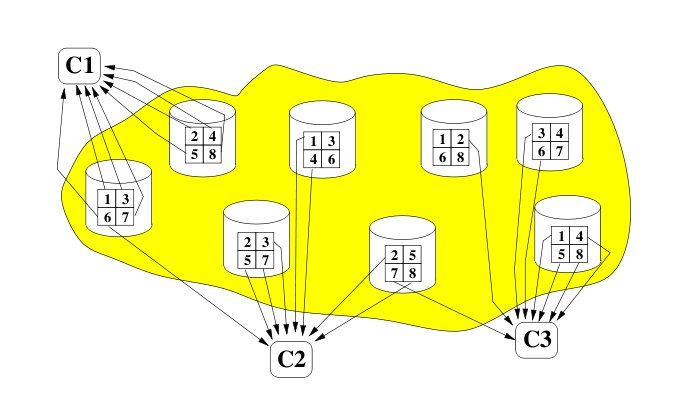
\includegraphics[scale=.6]{figuras/replicacao-pura.jpg}
     \caption{Sistema com replica��o pura \cite{Plank:2004}}
     \label{fig4:srp}
   \end{figure}

   \begin{figure}[h]
     \centering
     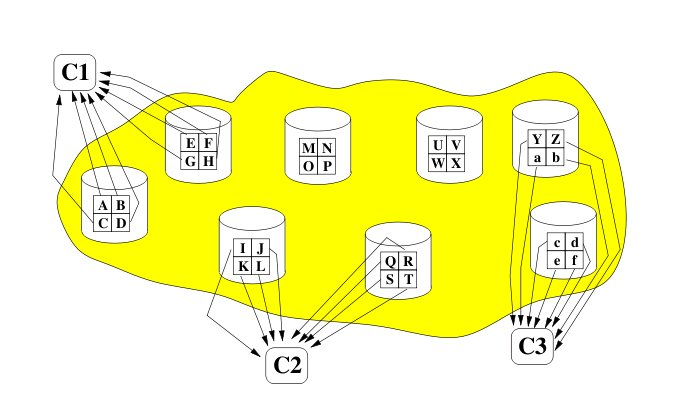
\includegraphics[scale=.6]{figuras/codigos-RS.jpg}
     \caption{Sistema com c�digos RS \cite{Plank:2004}}
     \label{fig5:crs}
   \end{figure}

\subsection{Replica��o}

Replica��o � o esquema de redund�ncia mais simples. A maioria dos sistemas, que utiliza redund�ncia de dados, � baseada em replica��o, mas esse esquema consume mais espa�o que a codifica��o por apagamento, pois uma c�pia completa de cada arquivo � armazenada em cada um dos servidores de dados.

A principal desvantagem da replica��o � que ela requer um grande \emph{overhead} de armazenamento para pouco ganho em disponibilidade e toler�ncia a falhas. Garantir que os dados permane�am dispon�veis quando todos os $n$ dispositivos falham exige que, pelo menos, $n + 1$ c�pias existam \cite{Woitaszek:2007}. Por exemplo, no artigo sobre o sistema Glacier \cite{Haeberlen:2005}, os autores argumentam que o armazenamento aumenta de 11 vezes a quantidade de dados armazenados utilizando apenas replica��o para conseguir 0.999999 (\emph{six nines}) de confiabilidade num cen�rio com 60\% de indisponibilidade dos \emph{peers}.

Os autores em \cite{Dabek:2004} afirmam que dados replicados permitem leituras de baixa lat�ncia, porque h� muitas op��es para a sele��o de servidores, enquanto que dados codificados reduzem o consumo de largura de banda para escritas, em detrimento do aumento da lat�ncia de leituras.

A replica��o � usada no Google File System \cite{Ghemawat:2003} (GFS), no Hadoop Distributed File System \cite{Hadoop:2010} (HDFS) e no Kosmos distributed file system \cite{TKDFS:2011} (KFS), sistemas de arquivos distribu�dos que apresentam caracter�sticas semelhantes. Um \emph{cluster} do GFS ou do HDFS ou do KFS � formado por um �nico servidor, master (GFS) ou namenode (HDFS) ou Meta server (KFS), que mant�m os metadados e muitos servidores de dados, os chunkservers (GFS e KFS) ou os datanodes (HDFS) e � acessado por v�rios clientes. Os arquivos de dados s�o armazenados nos chunkservers (GFS e KFS) ou datanodes (HDFS) e s�o particionados em blocos de igual tamanho. GFS, HDFS e KFS foram projetados para aplica��es que processam grande volume de dados. 

Seus projetos consideram \emph{clusters} de (\emph{commodity hardware}), uma vers�o do \emph{kernel} linux como sistema operacional para as m�quinas e uma arquitetura de rede com dois n�veis: v�rios \emph{racks} interligados por um comutador e cada \emph{rack} � formado por v�rias m�quinas e seus discos, estes tamb�m interligados por um comutador. A estrat�gia de inser��o de dados cria r�plicas em \emph{racks} distintos do \emph{rack} onde est� a 1$^a$ r�plica, assim, falhas que comprometam um \emph{rack} n�o provocam a indisponibilidade de dados. Os arquivos de dados s�o alterados por concatena��es ao inv�s de sobrescrever dados existentes. Ap�s a cria��o, os arquivos de dados s�o usados apenas para leitura e esta leitura ocorre sequencialmente. O KFS permite escrever em posi��es rand�micas nos arquivos. As APIs do cliente fornecidas pelo GFS, pelo HDFS e pelo KFS suportam opera��es de cria��o, leitura, escrita, remo��o de arquivos, mas n�o implementam a interface POSIX.

O GFS est� dispon�vel para linux sob uma licen�a de software propriet�rio. O HDFS \footnote{http://hadoop.apache.org/}  e o KFS \footnote{http://code.google.com/p/kosmosfs/} est�o dispon�veis para linux sob uma licen�a Apache. 

O Farsite, que utiliza apenas replica��o, � um sistema de arquivos distribu�dos, particionados em namespaces, explorando os desktops presentes dentro da Microsoft, sem servidor mestre, dispon�vel para Windows sob uma licen�a de software propriet�rio. A escolha da replica��o foi, pelos autores, considerada uma op��o mais simples para disponibilidade, j� que a codifica��o poderia significar lat�ncia adicional nas leituras dos arquivos. Ainda segundo os autores, estudos com experimentos j� mostraram que a codifica��o pode apresentar um bom desempenho e seria poss�vel, ent�o, alterar no futuro o esquema de redund�ncia do Farsite.

Big Table (constru�do sob o GFS) e Dynamo (constru�do para Amazon.com) s�o dois sistemas de armazenamento que gravam e recuperaram dados atrav�s de uma chave e executam em um \emph{pool} compartilhado de m�quinas, utilizam apenas replica��o. 

Ceph \cite{Weil:2006} � um sistema de arquivos \emph{open source} que possui tr�s principais componentes: um \emph{cluster} de servidores de metadados (que gerencia o namespace, nomes de arquivos e diret�rios), um \emph{cluster} de OSDs (dispositivos de armazenamento de objetos) que armazenam dados e metadados e os clientes que utilizam uma interface do sistema de arquivos. O Ceph agrupa dados em PGs (grupos de coloca��o) e usa uma fun��o \emph{hash} para distribuir os PGs nos OSDs, cujo algoritmo CRUSH � $O(log n)$ e usa uma �rvore-B para indexar os PGs. Existe um m�dulo em desenvolvimento que permite usar o Ceph como armazenamento para uma inst�ncia do Hadoop. O Ceph utiliza apenas replica��o, implementa parcialmente a interface POSIX e est� dispon�vel para linux sob LGPL \footnote{http://ceph.newdream.net/}.

Lustre \footnote{git://git.lustre.org/prime/lustre.git} tem na sua arquitetura os metadata server (disponibiliza os metadados para clientes), o metadata target (um por sistema de arquivos, armazena os metadados), object storage servers (armazena os dados), object storage target (armazena os objetos que cont�m os arquivos de dados) e clientes.

Moosefs \footnote{http://www.moosefs.org/} tamb�m foi projetado com uma arquitetura que se assemelha a do GFS, HDFS e KFS: master server (que armazena os metadados), chunk servers (que armazenam os dados), metalogger server (podem substituir algumas fun��es do master server, se ele falhar) e clientes (que solicitam dados e se comunicam com o master server e o chunk servers. 

Ambos, Lustre e Moosefs, usam replica��o, implementam a interface POSIX e est�o dispon�veis para linux sob uma licen�a GPL.

Com exce��o do Farsite, os sistemas de armazenamento apresentados consideram \emph{clusters} de (\emph{commodity hardware}) e uma vers�o do \emph{kernel} linux como sistema operacional para as m�quinas.

\subsection{Codifica��o por Apagamento}

Uma vantagem de codifica��o por apagamento � um custo menor de armazenamento se comparado a replica��o, no caso de grande volume de dados. Outra vantagem com rela��o a replica��o foi comentada em \cite{Weatherspoon:2002:01}: para um mesmo espa�o de armazenamento, o tempo m�dio entre falhas (\emph{mean time to failure}) � maior.

\begin{table}
%\singlespacing
    \centerline{
    \begin{tabular}{|p{2cm}|p{4cm}|p{5cm}|p{2cm}|}\hline
	{\bf sistema} & {\bf codifica��o} &  {\bf arquitetura do sistema} & {\bf licen�a}\\ \hline
	HDFS \cite{Hadoop:2010}& RAID, RS, ... & shared-disk file system for cluster & Apache\\ \hline
	Tahoe-LAFS \cite{Wilcox-O'Hearn:2008} \footnote{http://tahoe-lafs.org/trac/tahoe-lafs} & RAID & peer-to-peer filesystem & GPL2\\ \hline
	Pergamum \cite{Storer:2008}& XOR parity, RS &  disk-based archival storage & *\\ \hline
	Potshards \cite{Storer:2009} & RAID e RS &  disk-based archival storage & *\\ \hline
	RobuStore \cite{Xia:2006} & Luby Transform (LT) & disk-based archival storage & *\\ \hline
	Glacier \cite{Haeberlen:2005}& RS com matrizes Cauchy & peer-to-peer storage system & *\\ \hline
	Total Recall \cite{Bhagwan:2004} & Maymounkov's online codes &  peer-to-peer storage system & *\\ \hline
	FAB \cite{Saito:2004}& RS & distributed disk array & *\\ \hline
	GPFS \cite{Schmuck:2002}& RAID & shared-disk file system for cluster & *\\ \hline
	Oceanstore \cite{Kubiatowicz:2000} \footnote{http://oceanstore.sourceforge.net/}& Tornado e RS & desktops e notebooks conectados a servidores geograficamente distribu�dos & BSD \\ \hline
	xFS \cite{Anderson:1998} \footnote{http://oss.sgi.com/projects/xfs/} & RAID & serverless network file system & GPL\\ \hline
	Swift \cite{Cabrera:1991} & RAID & desktops sob unix conectados a uma intranet & *\\ \hline
    \end{tabular}}
    \caption{Compara��o de codifica��o entre sistemas de armazenamento de grande volume de dados que utilizam \emph{commodity hardware}}
    \label{tab1:comp}
    onde:\\
    * = n�o dispon�vel
\end{table}


HDFS, Total Recall e OceanStore usam codifica��o para reduzir o tamanho do armazenamento de dados e todos os outros sistemas usam codifica��o para prover disponibilidade e confiabilidade.

Os sistemas que foram comparados na tabela ~\ref{tab1:comp}, est�o dispon�veis para uma vers�o de sistema operacional linux ou unix. Al�m da codifica��o, todos eles implementam replica��o.

Vamos avaliar algumas das m�tricas utilizadas em literatura para comparar redund�ncia de dados em sistemas de armazenamento: sobrecarga de armazenamento, disponibilidade dos \emph{peers}, corrup��o de um dado e opera��es de cria��o, leitura, atualiza��o consistente e remo��o de dados redundantes. Inicialmente vamos definir alguns conceitos adaptados de \cite{Duminoco:2009, Chiola:2005, Rodrigues:2005, Williams:2007} para esses dois esquemas de redund�ncia.

\section{Caracteriza��o da replica��o e da codifica��o}

A confiabilidade de um esquema de redund�ncia � medida pelo n�mero de falhas simult�neas que ele pode tolerar sem comprometer a capacidade de reconstruir os dados originais. Assim esta propriedade pode ser expressada como a {\bf probabilidade de perda de dados, dado que ocorreram $l$ falhas}, $P(l)$.

Para avaliar o armazenamento, vamos definir {\bf fator de redund�ncia} $B$, uma raz�o entre tamanho dos dados originais mais a redund�ncia $|dado\ +\ red|$ e o tamanho dos dados originais $|dado|$ e tamb�m vamos definir grau de repara��o.

O {\bf grau de repara��o} mede o que deve ser feito ap�s parte da redund�ncia ser perdida. Para isso, � feita uma leitura de dados dispon�veis para produzir novos. O custo dessa leitura em um sistema de armazenamento distribu�do inclue volume do tr�fego da rede, pol�tica de repara��o, algoritmo de coordena��o. Nesse estudo vamos apenas avaliar a contribui��o do esquema de redund�ncia: a quantidade de dados a serem lidos para que dados novos sejam criados para reparar o dado corrompido, definido por $d$.

Definimos $p$ como a probabilidade de um \emph{peer} estar dispon�vel e  $q\ =\ 1\ -\ p$ como a probabilidade de um \emph{peer} n�o estar dispon�vel. Nesse estudo, assumimos que elas s�o iguais para todos os \emph{peers}.

Vamos definir as opera��es de acesso a dados redundantes como uma tupla $(r, w, a)$, onde $r$ � o n�mero m�nimo de \emph{peers} dispon�veis que armazenam dados redundantes, $w$ � o n�mero m�nimo de \emph{peers} dispon�veis que armazenam dados redundantes que devem ser acessados para armazenar novos valores e $a$ � n�mero de \emph{peers} (provavelmente outros) que devem estar dispon�veis para completar a opera��o.

\subsection{Replica��o}

Para as defini��es, $n$ � o n�mero de r�plicas dos dados.

{\bf n�mero de falhas suportadas} $l\ =\ n\ -\ 1$

{\bf probabilidade de perda de dados, dado que ocorreram $l$ falhas}

$$
P(l) = \left\{
\begin{array}{rcl}
0,& \mbox{se} & l\ <\ n\\
1,& \mbox{se} & l\ =\ n
\end{array}
\right.
$$

{\bf fator de redund�ncia}
$$
B\ =\ |dado\ +\ red|\ /\ |dado|\ =\ n
$$

{\bf grau de repara��o}
$$
d\ =\ 1
$$

{\bf disponibilidade de um dado}
$$
1 - q^n
$$

{\bf corrup��o de um dado}
$$
e = q^n
$$

\begin{table}
%\singlespacing
    \centerline{
    \begin{tabular}{|p{5cm}|p{5cm}|}\hline
        {\bf acesso} & {\bf tupla $(r, w, a)$}\\ \hline
        criar & $(0, 0, n)$\\ \hline
        apenas leitura & $(1, 0, 0)$\\ \hline
        atualiza��o consistente & $(1, n, 0)$\\ \hline
        apagar & $(0, n, 0)$\\ \hline
    \end{tabular}}
    \caption{Opera��es sobre dados redundantes na replica��o}
    \label{tab2:comp}
\end{table}

Comparando as tuplas (1, 0, 0) e (1, n, 0) da tabela ~\ref{tab2:comp}, podemos observar que a disponibilidade da opera��o "atualiza��o consistente" � menor que a disponibilidade da opera��o "apenas leitura", quando o n�mero de r�plicas $n > 1$ � aplicado.

\subsection{Codifica��o por Apagamento}

Na Codifica��o (m, k), $k$ � o n�mero de blocos originais do dado, $m$ � o n�mero de blocos codificados  e $m\ -\ k$ � o n�mero de blocos adicionados pela codifica��o.

{\bf n�mero de falhas suportadas} $l\ =\ m\ -\ k$

{\bf probabilidade de perda de dados, dado que ocorreram $l$ falhas}
$$
P(l) = \left\{
\begin{array}{rcl}
0,& \mbox{se} & l\ <=\ m\ -\ k\\
1,& \mbox{se} & l\ > m\ -\ k
\end{array}
\right.
$$

{\bf fator de redund�ncia}
$$
B\ =\ m / k
$$

{\bf grau de repara��o}
$$
d\ =\ k
$$

{\bf disponibilidade de um dado}
$$
B(k, m, p)\ =\ \sum_{i=k}^{m}{m \choose i}p^{i}q^{m-i}
$$

{\bf corrup��o de um dado}
$$
e = q^{m-k}
$$

\begin{table}
%\singlespacing
    \centerline{
    \begin{tabular}{|p{5cm}|p{5cm}|}\hline
       {\bf acesso} & {\bf tupla $(r, w, a)$}\\ \hline
       criar & $(0, 0, n)$\\ \hline
       apenas leitura & $(k, 0, 0)$\\ \hline
       atualiza��o consistente & $(k, m-k+1, k-1)$\\ \hline
       apagar & $(0, m-k+1, 0)$\\ \hline
    \end{tabular}}
    \caption{Opera��es sobre dados redundantes na codifica��o por apagamento}
    \label{tab3:comp}
\end{table}

Por outro lado, comparando-se as tuplas $(k, 0, 0)$ e $(k, m-k+1, k-1)$ da tabela ~\ref{tab3:comp}, podemos observar que existe um caso no qual as opera��es "apenas leitura" e "atualiza��o consistente" podem ter a mesma disponibilidade. Isto ocorre quando $m = 2k-1$ (assumindo-se tamb�m que n�mero total de \emph{peers} dispon�veis � maior ou igual a $m$), obtendo-se a tupla $(k, k, k-1)$.


\section{Sobrecarga de armazenamento}

Em \cite{Weatherspoon:2002:01, Dabek:2004}, os autores afirmam que a codifica��o obtem o mesmo n�vel de disponibilidade como a replica��o, usando muito menos espa�o de armazenamento.

Em \cite{Bhagwan:2004}, concluiu-se que se a disponibilidade do peer for 0.5, ent�o isso requer 10 c�pias de cada arquivo para garantir a disponibilidade de 0.999 dos arquivos.

No esquema da replica��o, para um objetivo de probabilidade de indisponibilidade de um dado $e = 0.0001$, dado uma probabilidade de um \emph{peer} estar indispon�vel $q = 0.05$, obtemos o valor de $n = 3$ r�plicas.

$$
\begin{array}{cl}
e\ =\ q^n\\
n\ =\ log\ e\ /\ log\ q\ =\ log\ 0.0001\ / log\ 0.05\ =\ 3.074487147\\
n\ \approx 3
\end{array}
$$

No esquema da codifica��o, para o mesmo objetivo, para as mesmas probabilidades $e$ e $q$, obtemos um valor de 4 blocos de paridade para uma codifica��o $(2k-1, k)$.
 
$$
\begin{array}{cl}
e\ =\ q^{m-k}\\
m\ -\ k\ =\ log\ e\ /\ log\ q
\end{array}
$$

Substituindo $m$ por $2k-1$ e $\ log\ e/\ log\ q$\ por $3.074487147$,
$$
\begin{array}{cl}
k-1\ =\ 3.074487147\\
k\ \approx\ 4 
\end{array}
$$

Para uma mesma probabilidade de indisponibilidade de um dado $e = 0.0001$ e uma mesma probabilidade de um \emph{peer} estar indispon�vel $q = 0.05$, obtemos o valor de $n = 3$ r�plicas para a replica��o e um valor de $k=4$ blocos iniciais para a codifica��o (2k-1,k). O fator de redund�ncia � $B\ =\ 3$ para a replica��o e $B\ =\ m / k\ =\ (2k-1) / k\ =\ 7/4\ =\ 1.75$ para a codifica��o.

No HDFS, a codifica��o RS \emph{default} � (5, 2) e a RAID-5 � (5, 3).  Logo, toleram at� $l=3$ e at� $l=2$ falhas, respectivamente, por \emph{stripe} de 5 blocos ($k=3$) com sobrecarga de $B=2.5$ e de $B=1,6667$, respectivamente.

Nas m�quinas do Facebook, a codifica��o RS � (13, 10) tem 10 blocos iniciais e 3 blocos de paridade ($B=1.3$) e a codifica��o RAID � (12, 10), 10 blocos iniciais e 2 blocos de paridade ($B=1.2$).

Na figura ~\ref{fig1:sarc}, podemos observar o gr�fico \footnote{O gr�fico foi gerado em formato PNG pelo Gnuplot.} das fun��es $y = 2x$, $y = 3x$ e $y = (2x-1)/x$, para $x>0$,  representando a sobrecarga de armazenamento na replica��o $2n$ e na $3n$ e na codifica��o $(2k-1,k)$, respectivamente. O eixo x representa o tamanho de um dado e o eixo y, a sobrecarga de armazenamento desse dado.

    \vspace*{2cm}
    \begin{figure}[h]
      \centering
      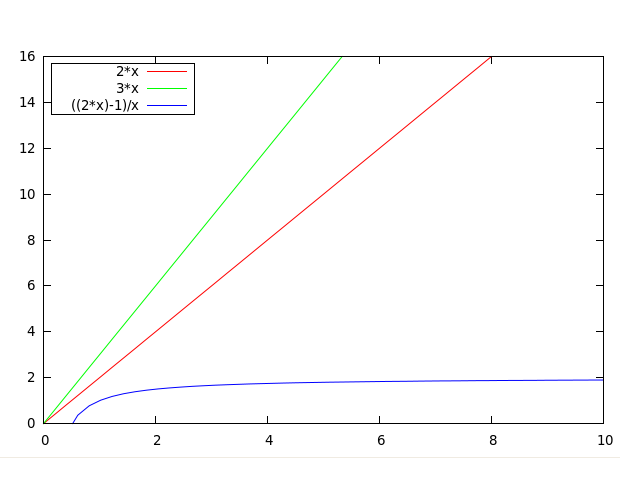
\includegraphics[scale=0.69]{figuras/gnuplot-replicacao-codificacao-3.png}
      \caption{Sobrecarga de armazenamento para replica��o $3n$, $2n$ e codifica��o $(2k-1,k)$ representadas, respectivamente, pelas fun��es $y = 3x$, $y = 2x$ e $y = (2x-1)/x$, para $x>0$}
      \label{fig1:sarc}
    \end{figure}

Neste estudo, conclu�mos que, apenas avaliando a contribui��o do esquema de redund�ncia, a codifica��o por apagamento acarreta uma sobrecarga de armazenamento menor que a replica��o para o mesmo n�mero de falhas toleradas. 

\section{Disponibilidade dos peers}

\section{Leitura ou Atualiza��o dos dados redundantes}

Em \cite{Chiola:2005}, os autores concluem que:

\begin{itemize}
  \item o acesso somente de leitura pode ser suportado tanto por replica��o de dados simples como por codifica��o
  \item para privilegiar atualiza��o consistente, uma codifica��o de alta disponibilidade � necess�ria que se caracteriza por fracionamento do original dados em peda�os $k$ e adicionando exatamente $k-1$ peda�os
  \item se ler e a disponibilidade de atualiza��o consistente s�o de igual import�ncia, isso requer codifica��o $(2k-1, k)$
\end{itemize}

Podemos tamb�m concluir que a replica��o � um caso onde $k = 1$ e $l\ =\ m - k\ = \ n\ -\ 1$, portanto $m\ =\ n$. 

Os autores tamb�m conclu�ram que usar apenas a replica��o tem sentido apenas em poucos casos.


    \chapter{Hadoop}

Atualmente, o Google � uma empresa de consulta e publicidade e � capaz de fornecer os seus servi�os devido a investimentos em armazenamento distribu�do em larga escala e a capacidade de processamento, estes desenvolvidos \emph{in-house}.

Essa capacidade � fornecida por um grande n�mero de PCs, pelo Google File System (GFS), um sistema de arquivos redundantes em \emph{cluster}, pelo sistema operacional GNU/Linux e pelo MapReduce, um \emph{middleware} de processamento paralelo de dados.

Em 2004, um artigo~\cite{Dean:2004}, que foi publicado por
profissionais da Google, prop�s o MapReduce. Em 2006, estes
profissionais, juntamente com Doug Cutting do Yahoo!, formaram um
sub-projeto do Apache Lucene\footnote{http://www.apache.org} que foi
chamado Hadoop\footnote{http://hadoop.apache.org/}.

Mais recentemente, o projeto Apache Hadoop tem desenvolvido uma
reimplementa��o de partes do GFS e MapReduce e muitos grupos da
comunidade de software livre posteriormente abra�aram essa tecnologia,
permitindo-lhes fazer coisas que eles n�o poderiam fazer em m�quinas
individuais. O Hadoop est� dispon�vel em c�digo fonte sob
licenciamento Apache \emph{license} (compat�vel com GPL).

O Hadoop � um \emph{framework} para executar aplica��es em
armazenamento distribu�do de grande volume de dados que pode ser
constru�do com \emph{commodity hardware}, que � facilmente acess�vel e
dispon�vel.  O Hadoop n�o � um \emph{framework} can�nico. Ele foi
projetado para aplica��es que atualizam dados da seguinte forma: uma
escrita e muitas leituras, atrav�s de acessos por \emph{batch}, com
tamanho da ordem de petabytes, organizados de forma n�o estruturada,
com esquema din�mico e integridade baixa.  Uma lista de aplica��es e
organiza��es que usam o Hadoop pode ser encontrada em
\cite{HadoopWiki:2010}.

Em poucas palavras, o Hadoop disponibiliza um armazenamento
compartilhado (HDFS) e um sistema de an�lise (MapReduce) que comp�em o
seu \emph{kernel}.

\section{MapReduce}

O MapReduce utiliza algoritmos de ordena��o para reconstruir sua base de dados.  Um bom uso para o MapReduce s�o aplica��es cujos dados s�o escritos uma vez e lidos muitas vezes. S�o dados n�o estruturados como texto ou imagens. O MapReduce tenta colocar esses dados no n� onde s�o feitas as computa��es, desta forma, o acesso aos dados � r�pido, pois � local \cite{White:2009}.

O MapReduce pode resolver problemas gen�ricos, cujos dados podem ser divididos em matrizes de dados, para cada matriz a mesma computa��o necess�ria (sub-problema) e n�o existe necessidade de comunica��o entre as tarefas (sub-problemas). A execu��o de um t�pico \emph{job} do MapReduce pode ser assim descrita:

\begin{itemize}
    \item Itera��o sobre um n�mero grande de registros
    \item Map extrai algo de cada registro (chave, valor)
    \item Rearranjo (\emph{shuffle}) e ordena��o de resultados intermedi�rios por (chave, valor)
    \item Reduce agrega os resultados intermedi�rios
    \item Gera��o da sa�da
\end{itemize}

Um programas para execu��o no HDFS/MapReduce que podem ser escritos em v�rias linguagens como Java, Ruby, Python e C++.


\section{Arquitetura do Hadoop \emph{Distributed File System}}

Um \emph{cluster} do HDFS � composto por um �nico NameNode, um
servidor-mestre que gerencia o sistema de arquivos e controla o acesso
aos arquivos de clientes. H� uma s�rie de DataNodes, geralmente um por
n� do \emph{cluster}, que gerenciam o armazenamento anexado ao n� em
que s�o executados. A Figura~\ref{fig6:hfs} mostra o NameNode e os
DataNodes.

Uma t�pica arquitetura de rede em dois n�veis para um \emph{cluster}
Hadoop � constru�da por v�rios \emph{racks} interligados por um
comutador como mostra a Figura~\ref{fig5:hc}. Cada \emph{rack} por sua
vez � formado por v�rios n�s (m�quinas) e seus discos, estes tamb�m
interligados por um comutador.

    \vspace*{2cm}
    \begin{figure}[h]
      \centering
      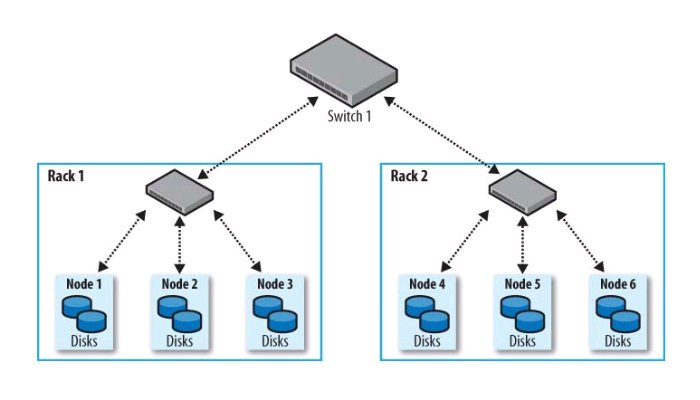
\includegraphics[scale=0.6]{figuras/hadoop-cluster.jpg}
      \caption{Arquitetura de rede em dois n�veis para um cluster Hadoop~\cite{Hadoop:2010}}
      \label{fig5:hc}
    \end{figure} 

O NameNode executa opera��es no sistema de arquivos, como \emph{open}, \emph{close}, \emph{rename} de arquivos e de diret�rios.

HDFS disponibiliza espa�o para sistema de arquivos e permite que os
dados do usu�rio sejam armazenados em arquivos. Internamente, um
arquivo � dividido em um ou mais blocos e esses blocos s�o armazenados
em um conjunto de DataNodes. A Figura~\ref{fig7:hfs} mostra DataNodes
e seus blocos. O tamanho \emph{default} de cada bloco � 64MB.

    \vspace*{2cm}
    \begin{figure}[h]
      \centering
      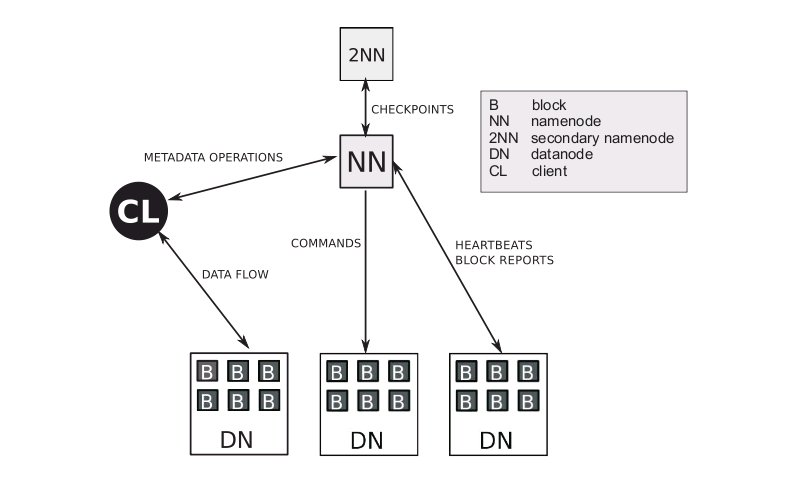
\includegraphics[scale=.6]{figuras/HDFS-arquitetura-2.jpg}
      \caption{Arquitetura do HDFS \cite{TR-IC-10-24}}
      \label{fig6:hfs}
    \end{figure} 

Os DataNodes respondem aos pedidos de leitura e escrita de clientes do
sistema de arquivos e tamb�m executam a cria��o, elimina��o e
replica��o de blocos sob instru��o do NameNode. O n�mero de r�plicas �
geralmente 3. A 1$^a$ r�plica fica local, no mesmo n� do c�digo do
cliente. A 2$^a$ r�plica fica em um n� em outro \emph{rack} e a 3$^a$
r�plica fica nesse �ltimo \emph{rack} em outro n�. As 2$^a$ e 3$^a$
r�plicas n�o s�o locais ao bloco replicado.

O NameNode e DataNode s�o partes do \emph{software} projetado para
rodar em \emph{commodity hardware}. Essas m�quinas normalmente
executam um sistema operacional GNU/Linux.

HDFS � constru�do usando a linguagem Java. Qualquer m�quina que suporte
Java pode executar o NameNode ou o DataNode \cite{Hadoop:2010}.

\vspace*{2cm}
\begin{figure}[h]
  \centering
  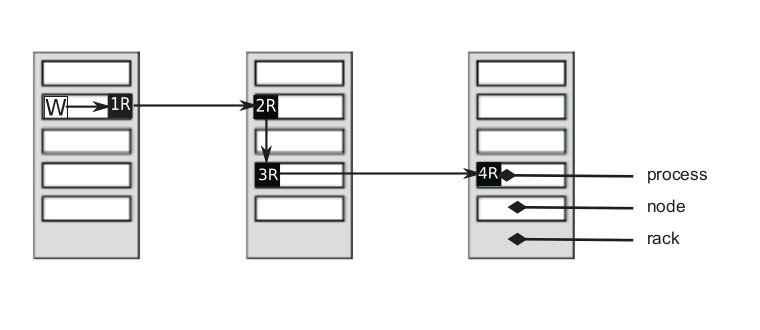
\includegraphics[scale=.5]{figuras/HDFS-arquitetura-replicacao-2.jpg}
  \caption{Arquitetura do HDFS - Datanodes e Blocos \cite{White:2009}}
  \label{fig7:hfs}
\end{figure} 

Os protocolos do HDFS usam o protocolo TCP/IP. O cliente fala o
protocolo ClientProtocol com o NameNode atrav�s de uma porta. Os
DataNodes falam o protocolo DataNodeProtocol com o NameNode. Esses
protocolos executam uma \emph{Remote Procedure Call} (RPC). O NameNode
n�o inicia chamadas RPCs. Ele responde a chamadas RPCs feitas pelo
DataNodes e pelos clientes.

\section{Codifica��o por Apagamento}

Existe uma nova caracter�stica proposta em 2009 para implementa��o de
uma camada de codifica��o por apagamento no Hadoop utilizando
XOR (RAID-5)~\cite{HDFS-503:2010} e uma mais recente utilizando c�digos
RS~\cite{MR-1969:2010}. A inclus�o da codifica��o por apagamento foi proposta com o
objetivo de reduzir o tamanho do armazenamento do HDFS.

A vers�o atual do Hadoop n�o utiliza apenas a t�cnica de replica��o
\cite{White:2009} para obter disponibilidade e confiabilidade de
dados. Ela pode ser configurada para usar tamb�m  codica��o XOR (RAID-5) e RS.

No HDFS, a codifica��o RS \emph{default} � (8, 5) e a XOR \emph{default} � (6, 5).  Logo, toleram at� $l=3$ e at� $l=1$ falhas, respectivamente, por \emph{stripe} de 5 blocos ($k=5$) com sobrecarga de $B=1.6$ e de $B=1.2$, respectivamente.

Na codifica��o XOR, � poss�vel configurar o n�mero de blocos por \emph{stripe}. J� na codifica��o RS, tanto o n�mero de blocos por \emph{stripe} e como o n�mero de blocos de paridade s�o configur�veis.

\subsection{Algoritmos da Camada RAID}

Exemplo do algoritmo de codifica��o

O tamanho da \emph{stripe} � 5 blocos e existe um arquivo $/a/arquivo.txt$ com exatamente 5 blocos. Nesse caso, o algoritmo de codifica��o da camada RAID faz o seguinte:

\begin{verbatim}
bloco[0] = primeiro bloco
bloco[1] = segundo bloco
bloco[2] = terceiro bloco
bloco[3] = quarto bloco
bloco[4] = quinto bloco

bloco_paridade = iniciado com 0 em todos os bytes

para i de 0 at� n�mero de bytes em um bloco:
   para j de 0 at� 4:
      bloco_paridade = bloco_paridade xor bloco[j][i]

para i de 0 at� 4:
   escreva bloco_paridade no arquivo /raid/a/arquivo.txt
\end{verbatim}

\subsection{Algoritmos da Camada RS}

Exemplo do algoritmo de codifica��o

O tamanho da \emph{stripe} � 5 blocos, s�o 3 blocos de paridade, o polin�mio primitivo � $x^8 + x^4 + x^3 + x^2 + 1$ e existe um arquivo $/a/arquivo.txt$ com exatamente 5 blocos. Nesse caso, o algoritmo de codifica��o da camada RS faz o seguinte:

\begin{verbatim}
// polin�mio primitivo g representado por 285
g = x^8 + x^4 + x^2 + x + 1 
m = 8
k = 5
i = 0
L = m-k
j = 0

bloco[0] = primeiro bloco
bloco[1] = segundo bloco
bloco[2] = terceiro bloco
bloco[3] = quarto bloco
bloco[4] = quinto bloco

enquanto j >= L fa�a
   // para GF = 2
   // x^0 representado por 1; x^1 por 2; x^2 por 4; x^3 por 8; 
   // x^4 por 16; x^5 por 32; x^6 por 64; x^7 por 128;
   a = x^j
   i = 0
   bloco_paridade[j] = iniciado com 0 em todos os bytes
   enquanto i >= k fa�a
      r = novo bloco
      resto(g, a, bloco[i], r)
      bloco_paridade[j] = bloco_paridade[j] xor r
      i++
   j++
   
para j de 0 at� L
   escreva bloco_paridade[j] no arquivo /raidrs/a/arquivo.txt

resto (g, a , bloco, r)
   para i de 0 at� n�mero de bytes em um bloco:
      r[i] = resto(g, a, bloco[i])

resto (g, a, b)
retorna resto = (byte) rem (g(b), a(b))
   
\end{verbatim}

    \chapter{Implementa��o das Codifica��es}

Uma boa escolha de codifica��o para um canal depende da sobrecarga de armazenamento, do tamanho do bloco, da complexidade dos algoritmos de codifica��o e de decodifica��o e se uma eventual n�o detec��o de erros � aceit�vel. C�digos LDPC e Tornado s�o vers�teis para serem projetados para muitas op��es de tamanho do bloco e de sobrecarga de armazenamento e segundo muitos estudos, c�digos LDPC s�o a codifica��o que mais se aproxima do limite de Shannon (quantidade m�xima de dados transmitidos em um canal em bytes por segundo).

\section{Codifica��o Tornado}

A id�ia b�sica deste algoritmo da codifica��o Tornado est� descrita em \cite{Woitaszek:2007,Stoten:2011}.

O c�lculo do checksum de 64 bits foi feito para cada 100 bytes. Para um bloco de 64MB, o checksum � de 5.12MB.

A sobrecarga de armazenamento de checksum � $\frac{864}{800} = 1.08$. A sobrecarga da paridade � $\frac{2n}{n} = 2$. Portanto, a  sobrecarga total de armazenamento � $1.08*2 = 2.16$.

O n�mero de falhas suportadas � $l\ =\ numero\ de\ blocos\ da\ stripe\ =\ s$.

A opera��o mais custosa dos algoritmos � o c�lculo do $XOR$ entre 2 blocos de 64M. S�o $\frac{s}{2}$ opera��es, no caso de $s$ par e $\frac{n}{2}-1$ opera��es, no caso de $s$ �mpar. Nesse caso, podemos afirmar que os algoritmos s�o lineares no tamanho da entrada, ou seja, $O(s)$.

O grafo da codifica��o para uma \emph{stripe} de tamanho 10 blocos �:

\begin{verbatim}
1 0 0 0 0 0 0 0 0 0
1 1 0 0 0 0 0 0 0 0
0 1 1 0 0 0 0 0 0 0
0 0 1 1 0 0 0 0 0 0
0 0 0 1 1 0 0 0 0 0
0 0 0 0 1 1 0 0 0 0
0 0 0 0 0 1 1 0 0 0
0 0 0 0 0 0 1 1 0 0
0 0 0 0 0 0 0 1 1 0
0 0 0 0 0 0 0 0 1 1
\end{verbatim}


\subsection{Algoritmo de Codifica��o}

Apresentamos o algoritmo de codifica��o para uma \emph{stripe} de tamanho $s$ blocos e que gera $s$ blocos de paridade. 

\begin{verbatim}
// Ler o arquivo /a/arquivo.txt
para i de 0 at� s-1:
   bloco[i] = i-�simo bloco da stripe

para i de 0 at� s-1:
   se i = 0
   ent�o
      bloco_paridade[i] = bloco[i]
   sen�o
      bloco_paridade[i] = bloco[i-1] xor bloco[i]
   i++

para i de 0 at� s-1:
   escreva bloco_paridade[i] no arquivo /tor/a/arquivo.txt
\end{verbatim}

\subsection{Algoritmo de Decodifica��o}

O algoritmo de decodifica��o faz o seguinte:

\begin{verbatim}
// Ler  o arquivo  /tor/a/arquivo.txt
para i de 0 at� s-1:
   bloco_paridade[i] = i-�simo bloco de paridade da stripe

para i de 0 at� s-1:
   se i = 0
   ent�o
      bloco[i] = bloco_paridade[i]
   sen�o
      bloco$[i] = bloco_paridade[i] xor bloco[i-1]
   i++
\end{verbatim}

\section{Codifica��o Simples Turbo-\emph{Like}}

Esse algoritmo foi baseado nos estudos de \cite{Divsalar:1998,MacKay:2003} e � muito simples de entender. 

A sobrecarga total de armazenamento � $\frac{2n}{n}=2$.

O n�mero de falhas suportadas � $l\ =\ numero\ de\ blocos\ da\ stripe\ =\ s$.

A opera��o mais custosa dos algoritmos � o c�lculo do $XOR$ entre 2 blocos de 64M. S�o $s$ opera��es. Nesse caso, podemos afirmar que os algoritmos s�o lineares no tamanho da entrada, ou seja, $O(s)$.

O grafo da codifica��o para uma \emph{stripe} de tamanho 10 blocos na sequ�ncia $7, 1, 4, 8, 2, 5, 9, 3, 0, 6$:

\begin{verbatim}
0 0 0 0 0 0 0 1 0 0
0 1 0 0 0 0 0 1 0 0
0 1 0 0 1 0 0 0 0 0
0 0 0 0 1 0 0 0 1 0
0 0 1 0 0 0 0 0 1 0
0 0 1 0 0 1 0 0 0 0
0 0 0 0 0 1 0 0 0 1
0 0 0 1 0 0 0 0 0 1
1 0 0 1 0 0 0 0 0 0
1 0 0 0 0 0 1 0 0 0
\end{verbatim}


\subsection{Algoritmo de Codifica��o}

Apresentamos o algoritmo de codifica��o para uma \emph{stripe} de tamanho $s$ blocos e que gera $s$ blocos de paridade.

\begin{verbatim}
// Ler o arquivo /a/arquivo.txt
para i de 0 at� s-1:
   bloco[i] = i-�simo bloco da stripe

Gerar uma permuta��o dos �ndices dos blocos da stripe: p = [b_0,
b_1, b_2, b_3, ..., b_{s-2}, b_{s-1}]

para i de 0 at� s-1:
   se p[i] = 0
   ent�o
      bloco_paridade[i] = bloco[p[i]]
   sen�o
      bloco_paridade[i] = bloco_paridade[i-1] xor bloco[p[i]]
   i++

para i de 0 at� s-1:
   escreva bloco_paridade[i] no arquivo /tor/a/arquivo.txt
\end{verbatim}

\subsection{Algoritmo de Decodifica��o}

O algoritmo de decodifica��o faz o seguinte:

\begin{verbatim}
Ler a permuta��o do �ndices dos blocos da stripe: p =  [b_0,
b_1, b_2, b_3, ..., b_{s-2}, b_{s-1}]

// Ler  o arquivo  /turbo/a/arquivo.txt
para i de 0 at� s-1:
   bloco_paridade[i] = i-�simo bloco de paridade da stripe

para i de 0 at� s-1:
   se p[i] = 0
   ent�o
      bloco[p[i]] = bloco_paridade[i]
   sen�o
      bloco[p[i]] = bloco_paridade[i-1] xor bloco_paridade[i]
   i++
\end{verbatim}

\begin{table}
%\singlespacing
    \centerline{
    \begin{tabular}{|p{3cm}|p{1.5cm}|p{1.5cm}|p{1.2cm}|p{2cm}|p{1.7cm}}\hline
	{\bf Codifica��o} & {\bf N�mero de falhas suportadas} &  {\bf Espa�o de armazenamento} & {\bf Grau de reparacao} & {\bf Corrup��o de um dado} & {\bf Complexidade dos algoritmos}\\ \hline
	Replica��o 2X & $l=2$ & $B=2$ & $d=1$ & $e = q^2$ & $O(1)$\\ \hline
	RAID (6, 5) & $l=1$ & $B=1.2$ & $d=5$ & $e = q$ & $O(5log 6)$\\ \hline
	RS (8, 5) & $l=3$ & $B=1.6$ & $d=5$ & $e = q^3$ & $O(5(3 log 8))$\\ \hline
	Tornado (10, 5) & $l=5$ & $B=2$ & $d=5$ & $e = q^5$ & $O(10)$\\ \hline
	Turbo-\emph{Like} (10, 5) & $l=5$ & $B=2$ & $d=5$ & $e = q^5$ & $O(10)$\\ \hline
	Replica��o $nX$ & $l=n$ & $B=n$ & $d=1$ & $e = q^{n-1}$ & $O(n)$\\ \hline
	RS $(2k, k) ou (2k-1,k)$ & $l=k$ & $B=2$ & $d=k$ & $e = q^k$ & $O(k^2log 2k) \cite{Luby:2002}$\\ \hline
	Tornado $(2k, k) ou (2k-1,k)$ & $l=k$ & $B=2$ & $d=k$ & $e = q^k$ & $O(2k) \cite{Luby:2002}$\\ \hline
	Turbo-\emph{Like} $(2k, k) ou (2k-1, k)$ & $l=k$ & $B=2$ & $d=k$ & $e = q^k$ & $O(2k)$\\ \hline
    \end{tabular}}
    \caption{Compara��o entre as codifica��es implementadas (nem todas ainda!) no HDFS}
    \label{tab2:comp}
\end{table}



    \chapter{Conclusões}


\section{Trabalhos Futuros}

\begin{itemize}

   \item A discussão sobre sobre esquemas adequados de redundância de dados do Capítulo 4 pode ser extendida através do teorema de Shannon-Hartley. Esse teorema afirma que um sistema com largura de banda a maior possível tem uma capacidade de canal finita. Em esboços preliminares, comparando-se,  para uma dada codificação, a probabilidade de erro em uma palavra código sem codificação com a probabilidade de erro em uma palavra código com codificação, pode-se chegar a conclusão que a probabilidade de erro em uma palavra código com codificação é menor que a probabilidade de erro em uma palavra código sem codificação.

\end{itemize}


    \bibliographystyle{plain}
    \bibliography{referencias/ref-dissertacao}
    \end{document}
